%\documentclass[review]{elsarticle}
%\documentclass[a4paper,fleqn,longmktitle]{cas-dc}
\documentclass[a4paper,fleqn]{cas-dc}\sloppy

%\usepackage[authoryear,longnamesfirst]{natbib}
%\usepackage[authoryear]{natbib}
\usepackage[numbers]{natbib}

\usepackage{hyperref}

% User for, well, math stuff
\usepackage{amsmath}

\usepackage[english,activeacute]{babel} 
\usepackage[toc,page]{appendix}
\usepackage{setspace}
\usepackage{graphics}
\usepackage{graphicx}
\usepackage{epsfig}
\usepackage{longtable}
\usepackage{steinmetz}
\usepackage{amsmath}
\usepackage{afterpage}
%\usepackage{indentfirst}
\usepackage{verbatim}
\usepackage{array}
\usepackage{amssymb}
\usepackage{fancyhdr}
\usepackage{mathrsfs}
\usepackage{lscape}
\usepackage[small,bf]{caption}
\usepackage{epstopdf}
\usepackage{alltt}
%\usepackage{siunitx}
\usepackage{caption}
\usepackage{rotating}
%\usepackage[hidelinks]{hyperref}
\usepackage{wrapfig}

\usepackage{subfigure}
\usepackage{verbatim}
\usepackage{color}
\usepackage{multirow}
\usepackage{float}
\usepackage[flushleft]{threeparttable}
\usepackage{hyperref}
\usepackage{longtable}
\usepackage{tensor}
\usepackage{listings}
\usepackage{color}
\usepackage{stackengine} 

\usepackage[utf8]{inputenc}

% command for co-polarized
\newcommand{\co}{\mathbin{\|}}
% command for cross-polarized
\newcommand{\cx}{\mathbin{\times}}

% symbol for spherical tensor convolution
\newcommand{\sconv}{\stackMath\mathbin{\stackinset{c}{0ex}{c}{0ex}{\ast}{\bigcirc}}}
\newcommand{\dsconv}{\stackMath\mathbin{\stackinset{c}{0ex}{c}{0ex}{\cdot}{\bigcirc}}}

%%%Author definitions
\def\tsc#1{\csdef{#1}{\textsc{\lowercase{#1}}\xspace}}
\tsc{WGM}
\tsc{QE}
\tsc{EP}
\tsc{PMS}
\tsc{BEC}
\tsc{DE}
%%%

\begin{document}
	
	\let\WriteBookmarks\relax
	\def\floatpagepagefraction{1}
	\def\textpagefraction{.001}
	\shorttitle{A PISCO for CMB experiments.}
	\shortauthors{Flux\'a et~al.}
	
	\title [mode = title]{Pixel space convolution for cosmic microwave background experiments}                      
	\tnotemark[1]
	\tnotetext[1]{This document is the results of the research project funded by FONDECYT ACBDE and ANILLO XXXX.}
	
	\author[1]{Pedro Flux\'a}
	{
		\fnmark[1]
		\ead[email]{pedro@fluxanet.net}
		\address[1]{Vicun\~na Mackenna 4860, Macul, RM, Santiago, Chile}
	}
	
	\author[2]{Michael K. Brewer}
	{
		\fnmark[2]
		%\ead[email]{rdunner@astro.puc.cl}
		%\address[2]{Vicun\~na Mackenna 4860, Macul, RM, Santiago, Chile}
	}	
	
	\author[3]{Rolando D\"unner}
	{
		\fnmark[3]
		\ead[email]{rdunner@astro.puc.cl}
		\address[3]{Vicun\~na Mackenna 4860, Macul, RM, Santiago, Chile}
	}
	
	\fntext[fn1]
	{
		Instituto de Astrof\'isica UC, Pontificia Universidad Cat\'olica de Chile.
	}
	
	\fntext[fn2]
	{
		Johns Hopkins University, Baltimore MD, 21218, USA.
	}
	
	
	\begin{abstract}
		Cosmic microwave background experiments have experienced an exponential increase in complexity, data size and sensitivity. Current and future experiments aim at characterizing the B-mode power spectrum which, due to its faintness, will require extreme control over systematic effects. One of such effects might arise by the complex coupling between the telescope beam and its scanning strategy. In this work, we present a new software tool, the Pixel Space COnvolver, PISCO, capable of producing mock data streams for a general CMB experiment. We show results of an application of PISCO to the Cosmology Large Angular Scale Surveryor, and its Q-band telescope. Results show that beam eccentricity might cause a temperature to polarization leakage above $\ell \approx 50$. 
	\end{abstract}
	
	\maketitle
	
	% enable numbering of equations that considers the section number
	\numberwithin{equation}{section}
	
	\section{Introduction}
	
	The study of the cosmic microwave background (CMB) in the last few decades has lead to major advances in Cosmology. In particular, the study of the temperature and polarization anisotropy field has allowed us to achieve percent level constraints on cosmological parameters, favoring a universe dominated by cold dark matter plus a cosmological constant ($\Lambda$CDM), known today as the standard model of Cosmology {\color{red} (cite most relevant papers including WMAP and Planck)}. Current efforts are mostly focused on the polarization anisotropy field, as it promises to provide independent constraints on the very early stages of the Universe. At these very first moments, the leading theory claims that the Universe exponentially expanded nearly 60 e-folds in a process called Inflation, becoming the flat, homogeneous and isotropic Universe that we see today. If true, gravitational waves generated by this expansion would have later interacted with the surface of last scatter, leaving a unique imprint in the polarization field which should be observable today.
	
	CMB anisotropies form a Gaussian field on the sky, being nearly 10\% polarized. The latter can be modeled as a spin-2 field, which is separable in two orthogonal components: a curl-free component called E-mode, and a divergence-free component called B-mode. In the absence of gravitational waves, the polarization field would contain only E-modes, which would be partially turned into B-modes by gravitational waves acting during the epochs of recombination and reionization. The resulting B-mode field would be one or two orders of magnitude lower than the E-mode signal, being very faint and difficult to measure. Moreover, recent results show that this signal lies below other foreground signals like gravitational lensing distortions induced by the matter distribution and polarized emissions from the interstellar medium {\color{red}(add cites)}. Thus, detecting the primordial B-mode signal has become a major technical challenge.
	
	Another source of confusion are experimental systematic effects. The tremendous increase in sensitivity of CMB experiments have brought into stage a long list of instrumental and observational effects, which need to be properly incorporated into the data reduction process, as well as for the design of future experiments. Being this an extended signal on the sky, understanding effects the detailed polarized antenna response of the telescope, and how it gets convolved with the sky signal (scan strategy), is key, as it can directly affect the scientific results.
	
	The main beam is where most of the radiation is captured by the antenna, and thus the effects of the beam shape and polarization have been extensively studied. 
	%Analytic techniques
	It has been shown that symmetrical beams with smooth profiles can be analytically accounted for when computing the power spectra of CMB maps (see \cite{2003ApJS..148...39P}).
	However, beam asymmetries can produce leakage between temperature and polarization (T to P), or between E-modes and B-modes (P to P). The impact of these effects on the maps, power spectra and scientific results, as well as mitigation techniques, have been proposed by \cite{PhysRevD.77.083003, 2007MNRAS.376.1767O, 2015JCAP...03..048D}.
	
	The problem becomes much more complicated when sidelobes are included, forcing the use of numerical methods to understand their effects.
	Several of these techniques rely on harmonic space representations of the beam, the sky and the scan strategy (\cite{2001PhRvD..63l3002W,2000PhRvD..62l3002C}). Harmonic space algorithms can also exploit redundancies in the computation that allow Fast Fourier Transform (FFT) techniques to be used. An excellent description of FFT-based algorithms, as well an implementation and application to a realistic CMB experiment is given in \cite{2018arXiv180905034D}. On the other hand, pixel space algorithms can account for time-varying effects, like transient events on the sky model, modulation techniques and optical distortions. The work of \cite{2011ApJS..193....5M} describes such an implementation, and its application to the Planck satellite mission.
	
	%Planks approach ... 
	The Planck experiment developed Full Focal Plane (FFP) simulations (see \cite{2016A&A...594A..12P}). At the time they were performed, FFP simulations took more than four million CPU-hours on a world-class supercomputer, and required almost 18 TB of storage. FFP simulations included very detailed noise models of the Planck mission and helped, among other things, to provide excellent constraints on the the cosmological parameters and their associated statistical errors (see \cite{2016A&A...594A..13P}). FFP simulations showed that effort on improving tools aiming at simulating CMB experiments will become valuable for current and future missions.
	
	%O'dea approach ...
	
	
	
	In this work, we describe the algorithm and prototype implementation of a new CMB computer simulation code, the Pixel Space COnvolver (PISCO). PISCO has the capability of accounting for arbitrary shaped, time-varying beams and sky models. Full polarization treatment of the beam properties is based on the work presented in \cite{2007MNRAS.376.1767O}. PISCO also exploits the massively parallel architecture of Graphics Processing Units (GPU), via the CUDA platform, and was designed from scratch to take advantage of HPC environments.
	
	This paper is organized as follows. 
	\S\ref{sec::coordinate-systems} contains a description of the coordinate system and geometrical transformations used to model an antenna pointing at the sky.
	\S\ref{sec::antennas} presents a brief introduction to antenna theory. 
	\S\ref{sec::pixel_conv} describes the algorithm used by PISCO, as well as a prototype implementation. 
	\S\ref{sec::validation} presents validation tests to assess the performance of PISCO. 
	\S\ref{sec::class_pisco_sim} provides an example application of PISCO to CLASS (\cite{2016SPIE.9914E..1KH}). 
	The paper concludes with a brief discussion on the results obtained in \S\ref{sec::conclusions}.
	
	%
	\section{Coordinates}
	\label{sec::coordinate-systems}
	
	\subsection{Definitions}
	
	\begin{figure*}
		\centering
		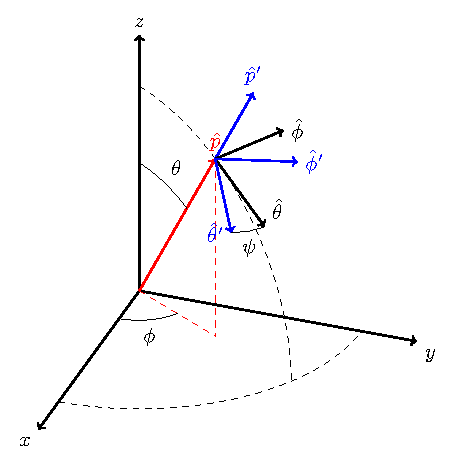
\includegraphics[width=0.43\linewidth]{tikz/sky_basis}	
		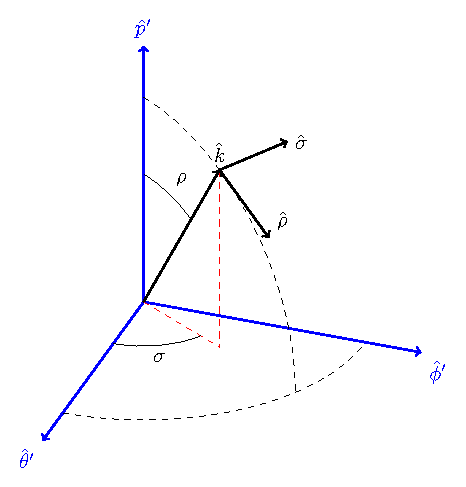
\includegraphics[width=0.43\linewidth]{tikz/beam_basis}
		\caption{Left panel: sky basis. The sky basis is a generic spherical coordinate system. $\hat{x}$, $\hat{y}$ and $\hat{z}$ form an orthonormal basis. Unit vector $\hat{p}$ is defined by its spherical coordinates, co-latitude $\theta$ and longitude $\phi$. Co-latitude increases from the north pole towards the south pole. Longitude increases from west to east. Tangent vectors at $\hat{p}$, $\hat{\theta}$ and $\hat{\phi}$, can be rotated around $\hat{p}$ by angle $\psi$ to generate vectors $\hat{\theta}'$ and $\hat{\phi}'$. Note an observer looking towards the sky along $\hat{p}$ will measure angle $\psi$ as increasing clockwise from South. Right panel: antenna basis. The antenna basis is another orthonormal basis, very much like the sky basis. A unit vector $\hat{k}$ is described by $\rho$ (co-latitude) and $\sigma$ (longitude). Tangent vectors at $\hat{k}$ are $\hat{\rho}$ and $\hat{\sigma}$. }
		\label{fig::sky_basis} 
	\end{figure*}
	
	In this work, we will use a spherical coordinate system described in figure \ref{fig::sky_basis}. We start by defining the \textsl{sky basis}, a coordinate system whose unit base vectors are $\hat{x}$, $\hat{y}$ and $\hat{z}$. For convenience, we will denote the antenna pointing as a 3-tuple $\bar{q}$ so that an antenna aiming at co-latitude $\theta_0$ and longitude $\phi_0$, with position angle $\psi_0$ has a pointing 
	
	\begin{equation}
	\begin{aligned}
	\bar{q}_0= (\theta_0,\phi_0,\psi_0)
	\end{aligned}
	\end{equation}
	
	The \textsl{pointing direction}, denoted by vector $\hat{p}$, can be expressed as a linear combination of base vectors and spherical coordinates $(\theta,\phi)$ via
	
	\begin{equation}
	\begin{aligned}
	\hat{p} = \cos(\phi)\sin(\theta)\hat{x} + \sin(\phi)\sin(\theta) \hat{y} + \cos(\theta) \hat{z}
	\end{aligned}
	\label{eq::p_sky_basis}
	\end{equation}
	
	Figure \ref{fig::sky_basis} shows vectors $\hat{\theta}$ and $\hat{\phi}$ as well, which are computed using
	
	\begin{eqnarray}
	\begin{aligned}
	\hat{\theta} &=&  \cos(\theta) \cos(\phi) \hat{x} + \cos(\theta)\sin(\phi) \hat{y} - \sin(\theta) \hat{z} \\
	\hat{\phi}   &=&              -\sin(\phi) \hat{x} +             \cos(\phi) \hat{y}
	\end{aligned}
	\label{eq::tangent_sky_basis}
	\end{eqnarray}
	
	These vectors can be used to build a second coordinate system, the \textsl{antenna basis}. Given an antenna pointing $\bar{q}$, the antenna basis base vectors can be written in term of sky basis coordinates as 
	
	\begin{eqnarray}
	%\begin{aligned}
	\hat{p}'      &=&  \hat{p} \\
	\hat{\theta}' &=&  \cos(\psi)\hat{\theta} + \sin(\psi)\hat{\phi} \\
	\hat{\phi}'   &=& -\sin(\psi)\hat{\theta} + \cos(\psi)\hat{\phi}
	%\end{aligned} 
	\label{eq::antenna_base_vectors}
	\end{eqnarray}
	
	In the antenna basis, coordinates analog to sky basis co-latitude and longitude are $\rho$ and $\sigma$, respectively. Similarly to equation \ref{eq::p_sky_basis}, a vector $\hat{k}$ can be written in terms of antenna basis coordinates as
	
	\begin{equation}
	\begin{aligned}
	\hat{k}       &=&  \cos(\sigma)\sin(\rho)\hat{\theta}_0' + \sin(\sigma)\sin(\rho) \hat{\phi}_0' + \cos(\rho) \hat{p}_0' \\
	\end{aligned}
	\end{equation}
	
	\noindent
	while vectors analog to the ones described by equation \ref{eq::tangent_sky_basis} are
	
	\begin{eqnarray}
	\begin{aligned}
	\hat{\rho}    &=&  \cos(\sigma)\cos(\rho)\hat{\theta}_0' + \sin(\sigma)\sin(\rho) \hat{\phi}_0' - \sin(\rho) \hat{p}_0' \\
	\hat{\sigma}  &=& -\sin(\sigma)\hat{\theta}_0' + \cos(\sigma)\hat{\phi}_0'
	\end{aligned}
	\end{eqnarray}
	
	In many situations, antennas are equipped with polarization sensitive devices. The direction on the sky for which the device has maximum sensitivity to linearly polarized radiation is called co-polarization, denoted by $\hat{e}_{\co}$. The perpendicular direction, known as cross-polarization, is denoted as $\hat{e}_{\cx}$.
	Both directions are defined in h Ludwig's third definition (see \cite{1140406}) provides a way of calculating both directions for a given point in the antenna basis, namely\footnote{The original definition differs from \ref{eq::ludwig} in that $\hat{\rho}$ must be swapped by $\hat{\phi}$.}
	
	\begin{eqnarray}
	\begin{aligned}
	\hat{e}_{\co} &=& \sin(\sigma) \hat{\sigma} + \cos(\sigma) \hat{\rho} \\
	\hat{e}_{\cx} &=& \cos(\sigma) \hat{\sigma} - \sin(\sigma) \hat{\rho} \, .
	\end{aligned}
	\label{eq::ludwig}
	\end{eqnarray}
	
	%\noindent
	Because polarization is defined in the sky basis (see Figure \ref{fig::cmbcoordconvention}), a polarization sensitive antenna must compensate for the apparent rotation of its own polarization basis with respect to the sky. This can me accomplished by rotating the incoming Stokes vector by the angle between $\hat{e}_{\co}$ and $\hat{\theta}$, namely
	
	\begin{equation}
	\chi(\rho,\sigma) = \arctan \left( \frac{ |\hat{e}_{\co} \times \hat{\theta}| }{ \hat{e}_{\co} \cdot \hat{\theta} } \right)
	\label{eq::chi}
	\end{equation}
	
	\begin{figure}
		\centering
		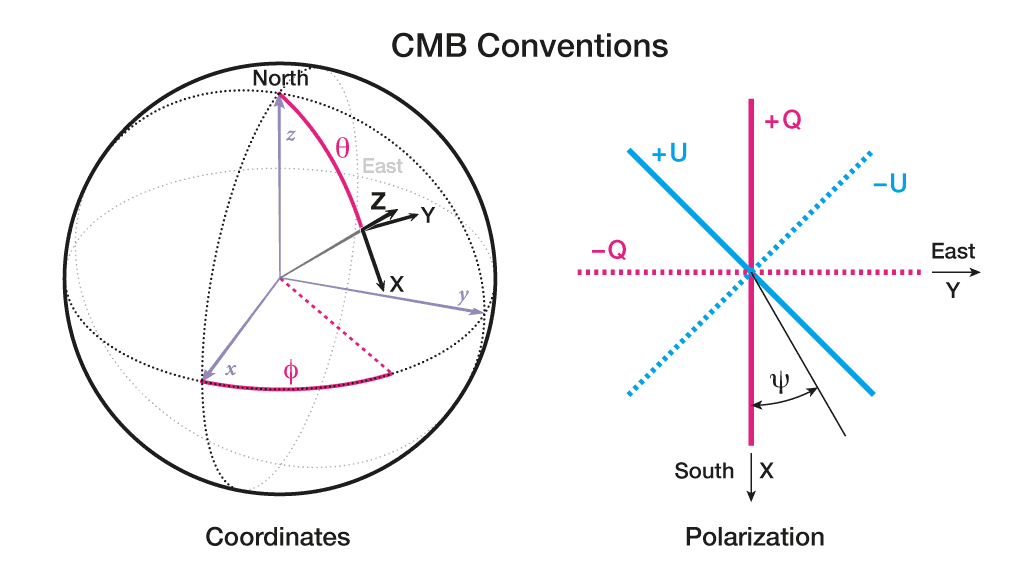
\includegraphics[width=1\linewidth]{figures/cmb_coord_convention}
		\caption{Figure showing the convention used for polarization among the CMB community. In this figure, $z$ is parallel to $\hat{p}_0$, $x$ is parallel to $\hat{\theta}$ and $y$ points along $\hat{\phi}$. $\psi$ is the angle between the antenna ``up'' direction, and $x$ ($\hat{\theta}$). The sign conventions of Stokes parameters $Q$ and $U$ used by the CMB community are: positive $Q$ if the polarization vector is aligned with $\hat(\theta)$ (North-South direction), negative $Q$ if the polarization vector is aligned with $\hat{\phi}$ (East-West direction), positive $U$ is aligned with $(\pm(\hat{\phi} - \hat{\theta})/\sqrt{2} )$ (North/East-South/West direction), and negative $U$ is parallel to $(\pm(\hat{\phi} + \hat{\theta})/\sqrt{2} )$ (North/West-South/East direction). Note that the right-most panel of this figure corresponds to an observer looking \textsl{towards Earth}. Figure source: \href{https://lambda.gsfc.nasa.gov/product/about/pol_convention.cfm}{LAMBDA website}}
		\label{fig::cmbcoordconvention}
	\end{figure}
	%
	%\subsection{The antenna basis}
	%
	%The reason to introduce the antenna basis is that physical properties of an antenna, like the beam, are described in a coordinate system that co-moves with the antenna. In turn, this coordinate system points to the sky along $\hat{p}_0$ with polarization sensitive angle $\psi_0$. To simplify the notation, we will consider the 3-tuple $\bar{p}_0$ to define the \textsl{antenna pointing}, as
	%
	%\begin{equation}
	%\begin{aligned}
	%\bar{p}_0 = (\theta_0,\phi_0,\psi_0)
	%\end{aligned}
	%\end{equation}
	%
	%\noindent
	%which should not be confused with the \textsl{antenna pointing direction}, $\hat{p}_0$.
	%
	%In order to model the process of observing the sky, relations between antenna and sky coordinates are needed. As described in figure \ref{fig::sky_basis}, vectors $\hat{x}'$ and $\hat{y}'$ are a rotation of tangent vectors at $\hat{p}_0$. Using Rodrigues' formula, we can express these vectors as
	%
	%\noindent
	%Together with $\hat{p}_0$, these vectors form the antenna basis. A vector $\hat{p}_0'$ can be written using antenna basis polar and azimuthal angles, $\rho_0$ and $\sigma_0$, via
	% 
	%\begin{equation}
	%\begin{aligned}
	%\hat{p}_0' = \cos(\sigma_0)\sin(\rho_0)\hat{x}' + \sin(\sigma_0)\sin(\rho_0) \hat{y}' + \cos(\rho_0) \hat{p}_0
	%\end{aligned}
	%\end{equation}
	%
	%\noindent
	%while the unit vectors analog to $\hat{\theta}$ and $\hat{\phi}$ at $\hat{p}_0'$ can also be defined as
	%
	%\begin{eqnarray}
	%\begin{aligned}
	%\hat{\rho}     &=&  \cos(\rho_0) \cos(\sigma_0) \hat{x}' + \cos(\rho_0)\sin(\sigma_0) \hat{y}' - \sin(\rho_0) \hat{p}_0 \\
	%\hat{\sigma}   &=&              -\sin(\sigma_0) \hat{x}' + \cos(\sigma_0)             \hat{y}'.
	%\end{aligned}
	%\end{eqnarray}
	%
	%\subsection{Relations between sky and antenna basis}
	%
	%Because $\hat{x}'$ and $\hat{y}'$ can be written in terms of sky basis vectors, all quantities defined in the antenna basis are uniquely related to their corresponding sky basis counterparts. Consider an antenna with pointing $\bar{p}_0$, and a sky basis vector with sky basis coordinates $(\theta,\phi)$. We can find the antenna basis spherical coordinates $(\rho,\sigma)$ that correspond to $(\theta,\phi)$ via operator $Z$ (see Appendix A), such that
	%
	%\begin{equation}
	%\begin{aligned}
	%\begin{bmatrix} 
	%\rho \\ 
	%\sigma 
	%\end{bmatrix} = Z( \theta,\phi ; \bar{p}_0 )
	%\label{eq::Z}
	%\end{aligned}
	%\end{equation}
	%
	%\noindent
	%For convenience, we consider $Z$ to return an antenna basis vectors if $(\theta,\phi)$ is replaced by a vector.
	%
	%\begin{equation}
	%\begin{aligned}
	%\hat{p}' = Z( \hat{p} ; \bar{p}_0 ).
	%\label{eq::Z_vec}
	%\end{aligned}
	%\end{equation}
	%
	%An observer measuring the CMB polarization field using an antenna will experience an apparent rotation of the polarization field. This is because $+Q$ in the sky basis is defined with respect to $\hat{\theta}$ while, in the antenna basis, it is defined with respect to $\hat{\rho}$. The angle $\Psi$ between $\hat{\rho}$ and $\hat{\theta}$ can be calculated as 
	%
	%\begin{equation}
	%\begin{aligned}
	%\Psi(\rho,\sigma; \theta,\phi, \bar{p}_0) = \arctan \left( \frac{ \hat{\rho} \times Z(\hat{\theta}) }{ \hat{\rho} \cdot Z(\hat{\theta}) } \right).
	%\label{eq::Psi}
	%\end{aligned}
	%\end{equation}
	%
	%\noindent
	%In the case of the CMB polarization field, $\Psi$ is used to transform Stokes parameters defined in the sky basis ($s$ subscript) to the antenna basis ($a$ subscript) via
	%
	%\begin{equation}
	%\begin{aligned}
	% \begin{bmatrix} 
	% I_a \\ 
	% Q_a \\ 
	% U_a \\ 
	% V_a 
	% \end{bmatrix}
	% =
	%\begin{bmatrix}
	%1 & 0 & 0 & 0 \\
	%0 & \cos(2\Psi) & \sin(2\Psi) & 0 \\
	%0 &-\sin(2\Psi) & \cos(2\Psi) & 0 \\
	%1 & 0 & 0 & 0
	%\end{bmatrix}
	%\cdot
	% \begin{bmatrix} 
	%I_s \\ 
	%Q_s \\ 
	%U_s \\ 
	%V_s 
	%\end{bmatrix}.
	%\end{aligned}
	%\label{eq::stokes_rotation}
	%\end{equation}
	%
	\section{Antenna theory}
	\label{sec::antennas}
	
	\subsection{Beam}
	
	The most fundamental property of an antenna is given by the angular distribution power density, $U(\rho,\sigma)$. For a lossless transmitting antenna broadcasting an amount of power $W$, we can write
	
	\begin{equation}
	\begin{aligned}
	W = \int_{4\pi} U(\rho,\sigma) \, \mathrm{d} \Omega \, .
	\end{aligned}
	\end{equation}
	
	\noindent
	The antenna beam is defined as
	
	\begin{equation}
	\begin{aligned}
	b(\rho, \sigma) = \frac{ U(\rho, \sigma) }{ \mathrm{MAX}\left[ U(\rho,\sigma) \right] }  =  \frac{ U(\rho, \sigma) }{ U(0,0) } \, .
	\end{aligned}
	\label{eq::beam_def}
	\end{equation}
	
	\noindent
	The beam also provides a quantification of how directional an antenna is, the beam solid angle $\Omega$, as
	
	\begin{equation}
	\begin{aligned}
	\Omega = \int_{4\pi} b(\rho,\sigma) \, \mathrm{d} \Omega \, .
	\end{aligned}
	\label{eq::omega_def}
	\end{equation}
	
	\subsection{Beam tensors}
	
	The Mueller matrix formalism is a vector-matrix framework that models the effect of optical elements in the polarization transfer function. The effect of an optical system with Mueller matrix $\mathbf{M}$ on a Stokes vector $S_{\mathrm{in}}$ is 
	
	\begin{equation}
	\begin{aligned}
	S_{\mathrm{out}} = \mathbf{M} S_{\mathrm{in}}
	\end{aligned}
	\end{equation}
	
	\noindent
	As described in the work of \cite{piepmeier_long_njoku_2008} and \cite{2007MNRAS.376.1767O}, antennas can also be modeled using Mueller matrices. This work is based on the work of \cite{2007MNRAS.376.1767O}, since it describes a formalism that is more suitable to be applied to CMB experiments. We note the original paper names ``beam Mueller fields'' to this extended definition of a antenna beam. In this work, we refer to it as a beam tensor, or \textsl{beamsor} for short.
	
	A beamsor can be interpreted as a field of Mueller matrices such that for each direction $(\rho,\sigma)$, there is an associated Mueller matrix that quantifies the coupling between the antenna and a Stokes vector coming from $(\rho,\sigma)$. We will denote a beamsor by letter $B = B(\rho,\sigma)$. At every antenna basis direction, $B$ is a $4\times4$ matrix in the form
	
	\begin{equation}
	\begin{aligned}
	B(\rho,\sigma) = \frac{1}{\tilde{\Omega}}
	\begin{bmatrix}
	B_{TT} & B_{QT} & B_{UT} & B_{VT}\\
	B_{TQ} & B_{QQ} & B_{UQ} & B_{VQ}\\
	B_{TU} & B_{QU} & B_{UU} & B_{VU}\\
	B_{TV} & B_{QV} & B_{UV} & B_{VV}
	\end{bmatrix}
	\end{aligned}
	\label{eq::beamsor}
	\end{equation}
	
	\noindent
	where $\tilde{\Omega}$ is a normalization factor
	
	\begin{equation}
	\begin{aligned}
	\tilde{\Omega} = \int_{4\pi} B_{TT}(\rho,\sigma) \, \mathrm{d} \Omega
	\end{aligned}
	\end{equation}
	
	\noindent
	and the elements of $B$ are defined in Appendix B. 
	
	%This is accomplished by considering that the electric fields resulting from propagating two orthogonal, linearly polarized sources through the antenna are known. Denoting the far-field component of the electric fields as by $\vec{E}_{\mathrm{x,y},\co}$ and $\vec{E}_{\mathrm{x,y},\co,\cx}$, and the sources by $x$ and $y$, the elements of the beamsor can be calculated as
	%
	%\begin{eqnarray}
	%B_{TT}&=&\frac{1}{2}\left(\left|\vec{E}_{x}\right|^{2}+\left|\vec{E}_{y}\right|^{2}\right)\\
	%B_{TQ}&=&\frac{1}{2}\left(\left|\vec{E}_{x,\co}\right|^{2}-\left|\vec{E}_{x,\cx}\right|^{2} + \left|E_{y,\cx}\right|^{2}-\left|E_{y,\co}\right|^{2}\right)\\
	%B_{TU}&=&\frac{1}{2}\left(\vec{E}_{x,\co} E_{x,\cx}^{*} - E_{y,\co} E_{y,\cx}^{*}\right) + \mathrm{c.c.}\\
	%B_{TV}&=&\frac{1}{2}\mathrm{i}\left(\vec{E}_{x,\co}\vec{E}_{x,\cx}^{*} + \vec{E}_{y,\co} \vec{E}_{y,\cx}^{*}\right) + \mathrm{c.c.}\\
	%B_{QT}&=&\frac{1}{2}\left(\left|\vec{E}_{A}\right|^{2}-\left|\vec{E}_{B}\right|^{2}\right)\\
	%B_{QQ}&=&\frac{1}{2}\left(\left|\vec{E}_{x,\co}\right|^{2}-\left|\vec{E}_{x,\cx}\right|^{2}+\left|\vec{E}_{y,\co}\right|^{2}-\left|\vec{E}_{y,\cx}\right|^{2}\right)\\
	%B_{QU}&=&\frac{1}{2}\left(\vec{E}_{x,\co} \vec{E}_{x,\cx}^{*} + \vec{E}_{y,\co} \vec{E}_{y,\cx}^{*}\right)+\mathrm{c.c.}\\
	%B_{QV}&=&\frac{1}{2}\mathrm{i}\left( \vec{E}_{x,\co} E_{x,\cx}^{*} - E_{y,\co} E_{y,\cx}^{*}\right)+\mathrm{c.c.}\\
	%B_{UT}&=&\frac{1}{2}\left( -\vec{E}_{x,\co} \vec{E}_{x,\cx}^{*} + \vec{E}_{y,\cx} \vec{E}_{y,\co}^{*}\right)+\mathrm{c.c.}\\
	%B_{UQ}&=&\frac{1}{2}\left(-\vec{E}_{x,\co}\vec{E}_{y,\cx}^{*} - \vec{E}_{x,\cx} \vec{E}_{y,\co}^{*}\right)+\mathrm{c.c.}\\
	%B_{UU}&=&\frac{1}{2}\left(\vec{E}_{x,\co} \vec{E}_{y,\co}^{*} - \vec{E}_{x,\cx} \vec{E}_{y,\cx}^{*}\right)+\mathrm{c.c.}\\
	%B_{UV}&=&\frac{1}{2}\mathrm{i}\left(\vec{E}_{x,\co} \vec{E}_{y,\co}^{*} + \vec{E}_{x,\cx}\vec{E}_{y,\cx}^{*}\right)+\mathrm{c.c.}\\
	%B_{VT}&=&\frac{1}{2}\mathrm{i}\left(\vec{E}_{x,\co} \vec{E}_{y,\cx}^{*} - \vec{E}_{x,\cx}\vec{E}_{y,\co}^{*}\right)+\mathrm{c.c.}\\
	%B_{VQ}&=&\frac{1}{2}\mathrm{i}\left(\vec{E}_{\mathrm{x,\co}} \vec{E}_{y,\cx}^{*} + \vec{E}_{x,\cx} \vec{E}_{y,\co}^{*}\right)+\mathrm{c.c.}\\
	%B_{VU}&=&\frac{1}{2}\mathrm{i}\left(-\vec{E}_{x,\co} \vec{E}_{y,\co}^{*} + \vec{E}_{A,\cx} \vec{E}_{y,\cx}^{*}\right)+\mathrm{c.c.}\\
	%B_{VV}&=&\frac{1}{2}\left(\vec{E}_{x,\co} \vec{E}_{y,\co}^{*} + \vec{E}_{x,\cx} \vec{E}_{y,\cx}^{*}\right)+\mathrm{c.c.}
	%\end{eqnarray}
	%
	%\noindent
	%where c.c. stands for complex conjugate. 
	
	\subsection{Measuring the sky with antennas}
	
	Using the formalism described in \cite{2007MNRAS.376.1767O} has the advantage of using Mueller calculus to model the process by which a detector measures the sky using an antenna. Following \cite{2007A&A...470..771J}, a partially polarized, total power detection device corresponds to the following row-vector 
	
	\begin{equation}
	\begin{aligned}
	\tensor{D}{_{i}}(\zeta,\epsilon,s) = \frac{s}{2} \left[(1 + \epsilon), (1 - \epsilon)\cos(2\zeta), (1 - \epsilon)\sin(2\zeta), 0 \right]
	\end{aligned}
	\label{eq::M_pol}
	\end{equation}
	
	\noindent
	where $1 - \epsilon$ is the polarization efficiency, $s$ is the voltage responsivity of the detector and the angle $\zeta$ is the orientation of the sensitivity axis of the linear polarizer with respect to $\hat{e}_{\co}$ at beam center. The process of taking a total power measurement on a Stokes vector $\tensor{S}{^{i}}$ is then
	
	\begin{equation}
	\begin{aligned}
	d = \tensor{D}{_{i}} \tensor{S}{^{i}}
	\end{aligned}
	\label{eq::total_power_measurement}
	\end{equation}
	
	\noindent
	Taking $\tensor{S}{^{i}}$ as the convolution between a beamsor and the sky model, a measurement taken by linearly polarized total power detector coupled to an antenna which points along $\hat{p}$ is described by
	
	\begin{equation}
	\begin{aligned}
	d(\bar{q}) = \tensor{D}{_{i}}(\zeta,\epsilon,s) \int_{4\pi} \tensor{B}{^{i}_{j} } \left[ \tensor{\Lambda}{^{j}_{k} } \tensor{S}{^{k}} \right ] \, \mathbf{d} \Omega
	\end{aligned}
	\label{eq::total_power}
	\end{equation}
	
	\noindent
	where $(i,j) = T,Q,U,V$, and $B$ has been implicitly rotated so it is aligned according to $\bar{q}$ (see Appendix A). Rotation of the sky to antenna polarization basis is carried out by $\Lambda$, which is a matrix field in the form
	
	\begin{equation}
	\begin{aligned}
	\Lambda =
	\begin{bmatrix}
	1  & 0 & 0 & 0\\
	0  & \cos(2\chi) & \sin(2\chi) & 0\\
	0  &-\sin(2\chi) & \cos(2\chi) & 0\\
	0  & 0 & 0 & 1
	\end{bmatrix}
	\end{aligned}
	\label{eq::lambda_operator}
	\end{equation}
	
	%
	\section{Pixel space convolution}
	\label{sec::pixel_conv}
	
	\subsection{Discrete convolution on the sphere}
	
	It is convenient to consider a few conventions that will be used in this section. Continuous fields on the sphere are denoted using capital letters, like $F$. The $k$-th pixel of the pixelated counterpart of $F$ will be written as $\tensor[_k]{F}{}$. A useful interpretation of $\tensor[_k]{F}{}$ is to consider it as the $k$-th row in matrix of $N_p$ (number of pixels) sub-matrices. In this formalism, a pixelated beamsor would be represented by an $N_p \times 4 \times 4$ matrix.
	
	Pixelization of a function defined on the sphere can be modeled as a process where the continuous field $F = F(\theta,\phi)$ becomes a matrix. Generally, any pixelization scheme will make use of a pixel weighting function $w(\theta,\phi)$ to smooth rapid variations of $F$ inside the pixel domain. This is crucial to avoid aliasing noise, which can negatively impact harmonic space analysis of pixelated maps. In this context, to obtain the value of $\tensor[_k]{F}{}$ we must calculate the convolution of $k$-pixel weighting function with $F$, namely 
	
	\begin{equation}
	\begin{aligned}
	\tensor[_k]{F}{} = \int {}_k w (\theta,\phi) F(\theta,\phi) \, \mathrm{d} \Omega
	\end{aligned}
	\label{eq::howtopixelate}
	\end{equation}
	
	\noindent
	It is worth noting that PISCO does not explicitly compute equation \ref{eq::howtopixelate}, as the input maps which are used to generate TOD are already pixelated. The same situation applies for beamsors, which are also inputted as pixelated maps.
	
	Following the aforementioned conventions, the pixel space version of equation \ref{eq::total_power} becomes
	
	\begin{equation}
	\begin{aligned}
	d(\bar{q}) = \
	\tensor{D}{_{i}}(\zeta,\epsilon,s) \
	\sum_{k=1}^{N_p} \
	\tensor[_k]{B}{^i_j} \
	\tensor[_k]{\Lambda}{^j_m} \
	\tensor[_k]{S}{^m}
	\end{aligned}
	\label{eq::discrete_beam_conv_tensor}
	\end{equation}
	
	\noindent
	where we have implicitly assumed that $B$ has been properly re-pixelated so as to be aligned according to $\bar{q}$. 
	
	\subsection{Implementation in CUDA}
	
	GPUs allow for substantial acceleration of algorithms that perform a large amount of independent operations\cite{sanders2010cuda}. TOD generation using equation \ref{eq::discrete_beam_conv_tensor} is a great application case, because all operations are independent of each other, including the ones within a convolution. To better understand how this parallelism can exploited, consider the process of synthesizing $N_s$ measurements, each one associated with a pointing $\bar{p}_t$, using a CUDA grid of $B$ blocks and $T$ threads.
	
	The main algorithm consists of two nested loops, $L1$ and $L2$. $L1$ loops over the pointing, so that each block is associated with a given pointing direction. Note that this makes $L1$ execute $B$ operations in parallel. To prevent a race condition, the pointing is cloned $T$ times so that each thread in a block can read it from memory as fast as possible. $L2$ iterates on beamsor and sky pixel. Since every block executes $T$ threads, every block can compute $N_p/T$ partial summations of equation \ref{eq::discrete_beam_conv_tensor} in parallel. A third, higher level loop, can also be added to the algorithm to further chunk the pointing stream and make use of $N_g$ GPU instances. A graphical description of the algorithm is shown in figure \ref{fig::pisco_diagram}.
	
	\begin{figure}
		\begin{center}
			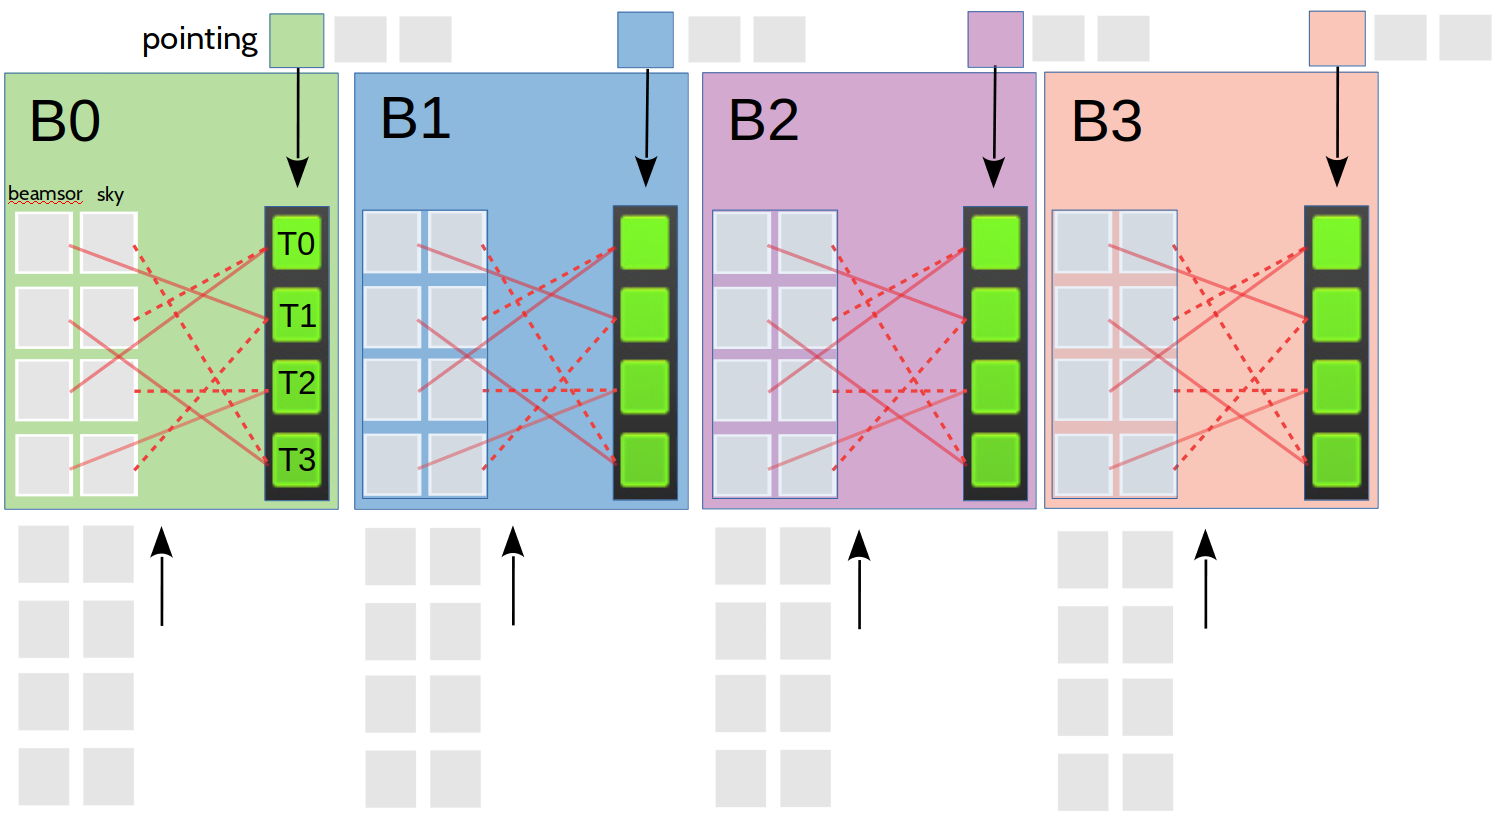
\includegraphics[width=1.0\linewidth]{figures/PISCO-diagram.png}
			\caption{Parallelization scheme. This figure shows the case of PISCO executing in 4 blocks ($B=4$), with four threads per block ($T=4$). Arrays with beamsor and sky elements are at the bottom. Each block has access to four beamsor and sky pixels (gray boxes inside colored boxes) and one pointing entry (colored small boxes) at a time. Green boxes represent the multiplication process of a single beamsor pixel with a single sky pixel. This includes rotating the sky pixel to the antenna polarization basis, and computing the repixelization of $B$ at the corresponding coordinates. Solid and dotted red lines represent the complex memory access pattern generated by this process. Every thread within a block writes its result to shared memory space. When a thread finishes its computation, it waits until all threads have finished and a reduction on the shared memory space is performed on across all blocks. This process is repeated for every pointing. At the end of the procedure, each block has computed the convolution of a beamsor with the sky for a particular pointing, and every shared memory space of the block has the corresponding result. These results are collected into the GPU global memory, which is then transferred back to CPU (host) memory.}
			\label{fig::pisco_diagram}
		\end{center}
	\end{figure}
	
	\subsection{PISCO}
	
	The \textbf{PI}xel \textbf{S}pace \textbf{CO}nvolver (PISCO) is a tool with the capability of generating synthetic Time Ordered Data (TOD) provided a model for the beamsor, the scanning strategy of the mission and a sky model. In this section, we present a pathfinder implementation of PISCO that makes use of the massively parallel architecture of modern GPU systems.
	
	\subsubsection{General description}
	
	PISCO is the software tool in charge of generating mock TOD given a beamsor, a sky model and a scanning strategy. A diagram showing the general workings of PISCO is shown in figure \ref{fig::pisco_flow}. PISCO receives as input a sky model in the form of 4 maps representing Stokes parameters $I,Q,U$ and $V$, a beamsor, pointing and focal plane information. The focal plane specifications are only needed if multiple detectors are being included in the pointing stream, as PISCO needs the the angle $\zeta$ of each detector to compute equation \ref{eq::discrete_beam_conv_tensor}. All the inputs are sent to the TOD generation function, which returns the data streams. At this point, the data can either be saved to disk or sent to a map-making code. This last step is preferred as, usually, input-output operations are time consuming. Finally, maps can be analyzed using external tools to calculate the power spectra.
	
	\begin{figure}
		\centering
		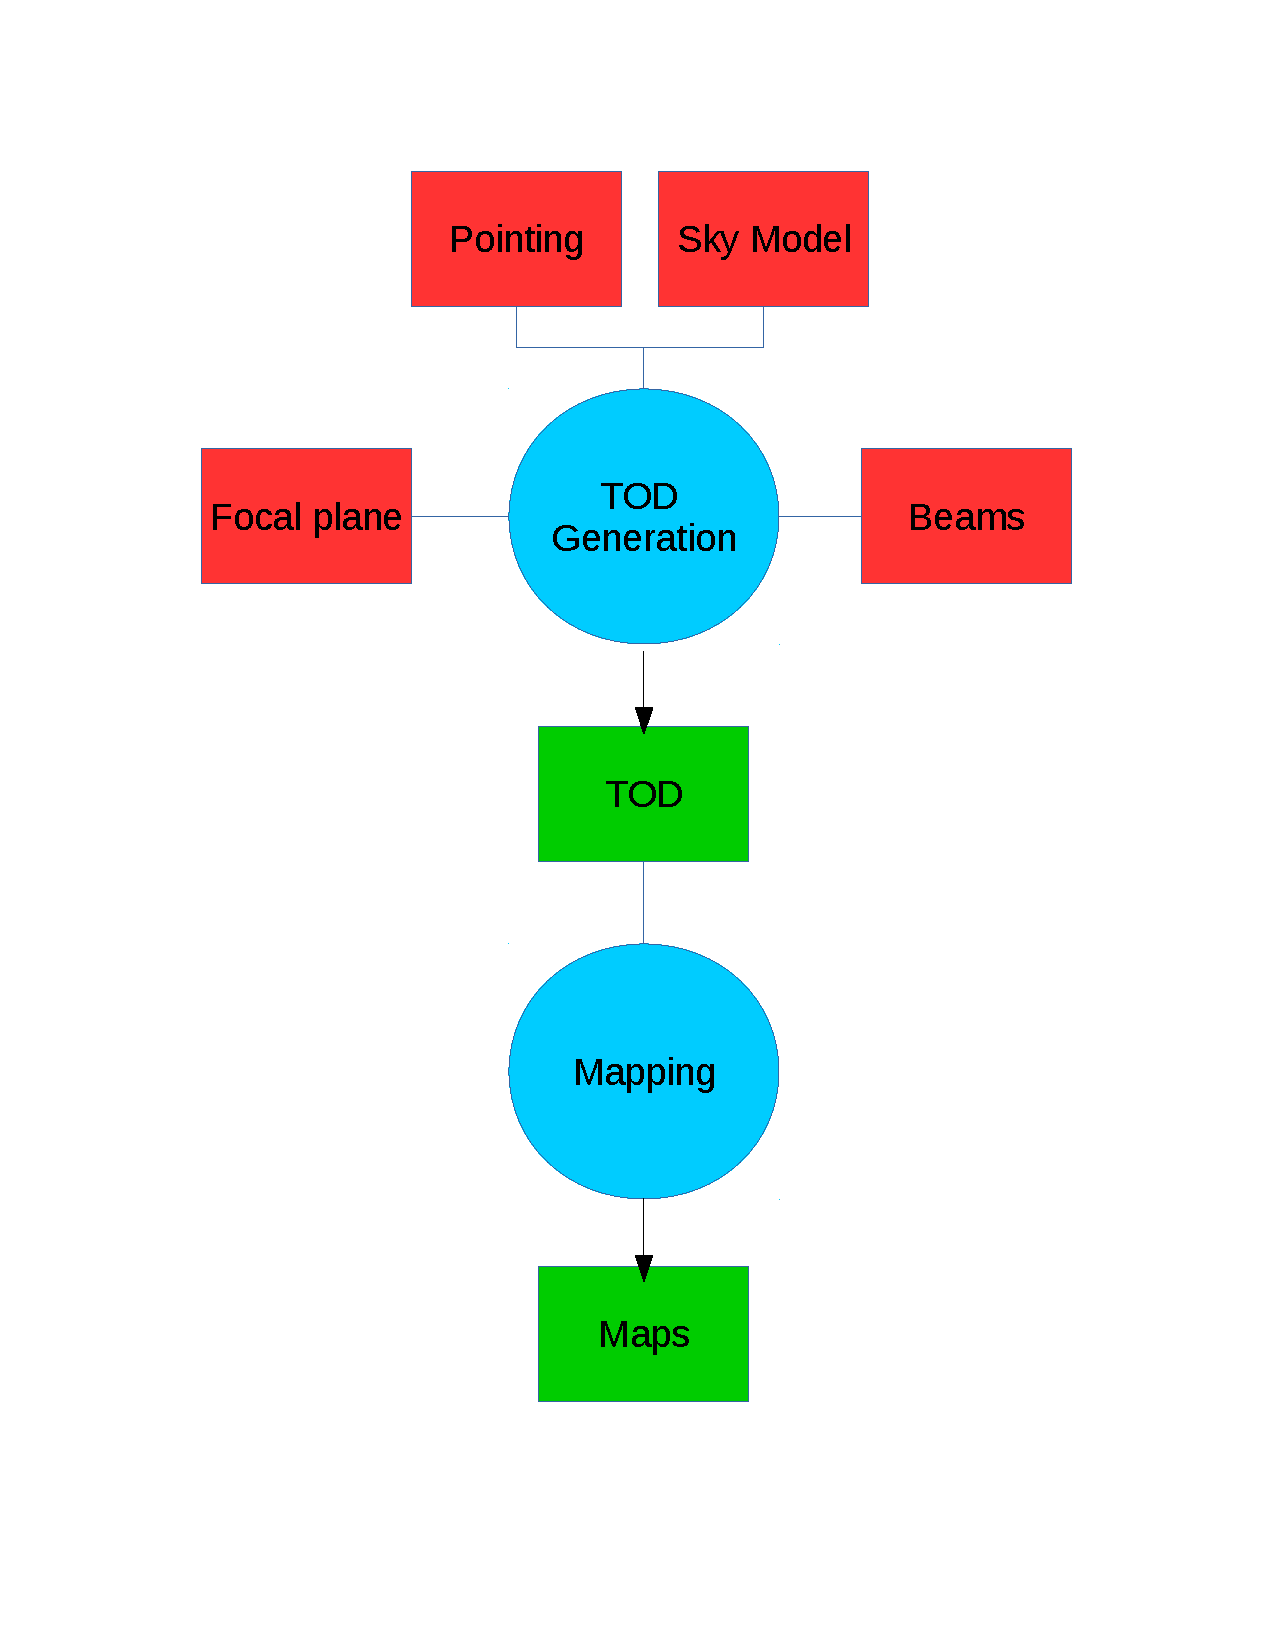
\includegraphics[width=1.0\linewidth]{figures/pisco-flow-diagram}
		\caption{Basic flow of a typical PISCO simulation pipeline. Red polygons show the required user input. PISCO uses this input and produces TOD (green polygon). This TOD stream is calculated using equation \ref{eq::discrete_beam_conv_tensor} for all pointing directions. TOD can then by sent into a mapper and, finally, to a power spectra estimator tool. PISCO does not compute pointing nor produces maps from TOD by itself; these tasks are left to external programs.}
		\label{fig::pisco_flow}
	\end{figure}
	
	\subsubsection{Performance}
	
	For large enough pointing streams, the available parallelism scales as $N_g \times B \times T$. We note that using larger pointing streams might affect performance, as reading from disc is usually slow. We believe that this penalty should be greatly suppressed by the use of a parallel file-system, which is a standard capability of modern HPC facilities. We also performed a test showing that the time spent loading a pointing stream with over 870 million data points takes less than $1\%$ of the overall execution time. Following the experience of FeBeCOP and TOAST, the current pipeline shown in figure \ref{fig::pisco_flow} does not write the mock TOD to disc.
	
	A realistic run took about 4 hours and 10 minutes on a single NVIDIA GTX 1080. The machine was also equipped with two Intel Xeon E5-2610 processors (20 physical cores, 40 threads). This run generated mock data for more than 870 million pointing directions. Each beamsor was represented by 5940 pixels. We note that this number only increases the accuracy of the re-pixelization step at the cost of increased memory requirements rather than any additional compute time. The actual number of pixels involved in a single convolution was 370 on average. The time taken by the map-making code is negligible compared to the convolution step, so it is not considered. With this particular simulation setup, PISCO was able to generate data 40 times faster than a real-time observation by computing more than 19 million convolutions per second. 
	
	The complex operations in the CUDA kernels involve large amounts of floating point and integer computations. This makes it difficult to estimate the performance as FLOPS. Also, the CUDA routine reads values from memory in a pseudo-random access pattern, something that is not efficiently performed by GPUs. The penalty associated with this situation is challenging to estimate. Finally, this implementation of PISCO pre-computes the cap of pixels around a given pointing direction in the CPU. While this process is fast, transferring the resulting memory buffer to the GPU takes as much as $30\%$ of the computation time. A solution to this problem has already been devised, and will be implemented in future releases.
	
	\begin{table}[width=.9\linewidth,cols=3,pos=h]
		\caption{Table summarizing the times taken by different routines of PISCO. The simulation executed at more than 19 million convolutions per second.}\label{tbl1}
		\begin{tabular*}{\tblwidth}{@{} LLLL@{} }
			\toprule
			Routine description & Time (in seconds) & $\%$ of total time \\
			\midrule
			convolution & 7967 & 52$\%$ & \\
			query pixel cap & 2171 & 14$\%$ & \\
			transfer pixel cap & 3978 & 27$\%$ & \\
			others & 985 & 7$\%$ & \\
			\bottomrule
		\end{tabular*}
	\end{table}
	
	%
	\section{Code validation}
	\label{sec::validation}
	
	\subsection{Validation using mock point source observations}
	
	The first test involved comparing the capability of PISCO to correctly reproduce observations of a point source at an arbitrary location on the sphere. The beamsor used in this test corresponded to the equivalent of a circularly symmetric Gaussian beam. The simulation setup can be summarized as
	
	\begin{itemize}
		\item Build a sky map with a single pixel with coordinates $(\theta_k,\phi_k)$ having a Stokes vector $S^{i} = (1,Q,U,0)$, such that $Q^2 + U^2 = 1$.
		\item Set up a raster scan around $(\theta_k,\phi_k)$ for a detector with $\zeta=0$. In order to have full polarization coverage, the scan is performed 3 times with angles $\psi_0 = 0^{\circ},45^{\circ},90^{\circ}$.
		\item Make maps of TOD generated by PISCO.
		\item Compare the maps with a harmonic space convolution of the single pixel map with the Gaussian beam.
	\end{itemize}
	
	\noindent
	Convolution in harmonic space was performed using the routines available in the HEALPix software package\cite{2005ApJ...622..759G}, particularly the \texttt{smoothing} routine provided by \texttt{healpy} Python wrapper. \texttt{smoothing} performs the harmonic space tensor convolution of a circularly symmetric Gaussian with a given sky model. In order to ease the comparison, TOD produced by PISCO were also projected to a HEALPix map. Since synthetic TOD are free of noise, an unweighted co-adding algorithm was used for map-making. We note that at least three observations at different position angles are needed in order to recover the Stokes parameters $I,Q$ and $U$ from each pixel.
	
	In order to find the optimal HEALPix resolution parameters for the beamsor and the sky, we used the prescription described in the FeBeCOP paper (see \cite{2011ApJS..193....5M}) as a starting point. This yielded a ``rule of thumb'' for the ratio $\mathrm{\texttt{NSIDE}}_{B} / \mathrm{\texttt{NSIDE}}_{S} = 4$ so that the convolution preserved the input map flux to better than $0.1\%$. We note that this flux mismatch is independent of the location of the point source, so its effect on whole sky maps should be a constant amplitude bias on the power spectra.
	
	Another important fact arises from considering the finite size of the beam (beamsor). When the antenna points near the poles, rapid variations of $\chi$ occur inside the beam. This becomes increasingly more problematic when reaching the poles. In order to correctly take this into account, the computation of $\chi$ used by PISCO was derived from first principles using spherical trigonometry, and the code was thoroughly tested and benchmarked to provide optimal performance. 
	
	\subsubsection{Results}
	
	Results from this validation test are shown in figure \ref{fig::stokesqsource256beam1024dec45}. The first test was to convolve the Gaussian beam with an unpolarized point source. The results show that the flux is preserved to better than $0.1\%$, as expected from using a beamsor-sky \texttt{NSIDE} ratio of 4. Finite machine precision produce leakage from temperature to polarization, but its amplitude is negligible: at least $10$ orders of magnitude below the maximum amplitude of the Stokes I convolved map. Similar results are obtained for polarized sources in $Q$ and $U$. In the case of polarized sources, however, the effect of in-beam variations of $\chi$ becomes dominant. This behavior was expected, and PISCO correctly reproduces the output of harmonic space convolution which naturally handles this situation.
	
	\begin{figure*}
		\centering
		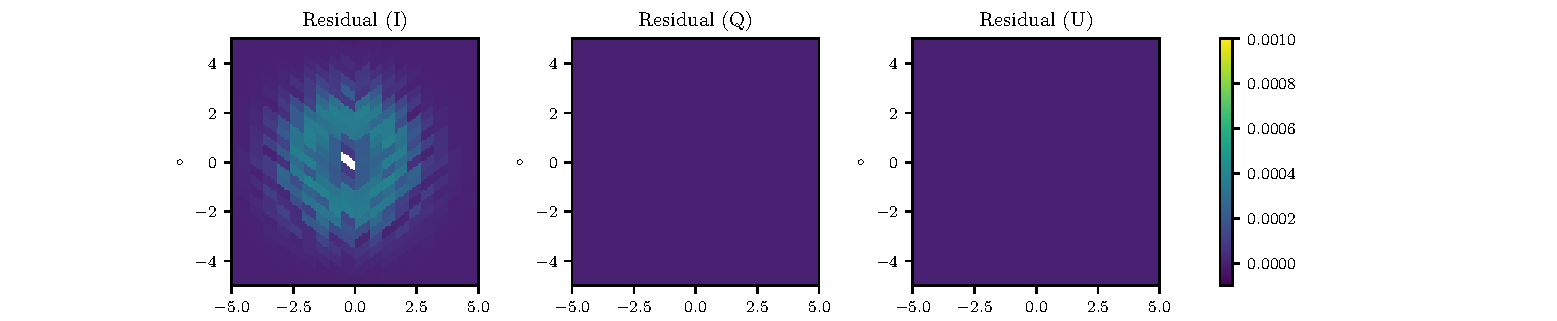
\includegraphics[width=1.0\linewidth]{figures/stokes_I_source_256_beam_1024_dec_45.pdf}
		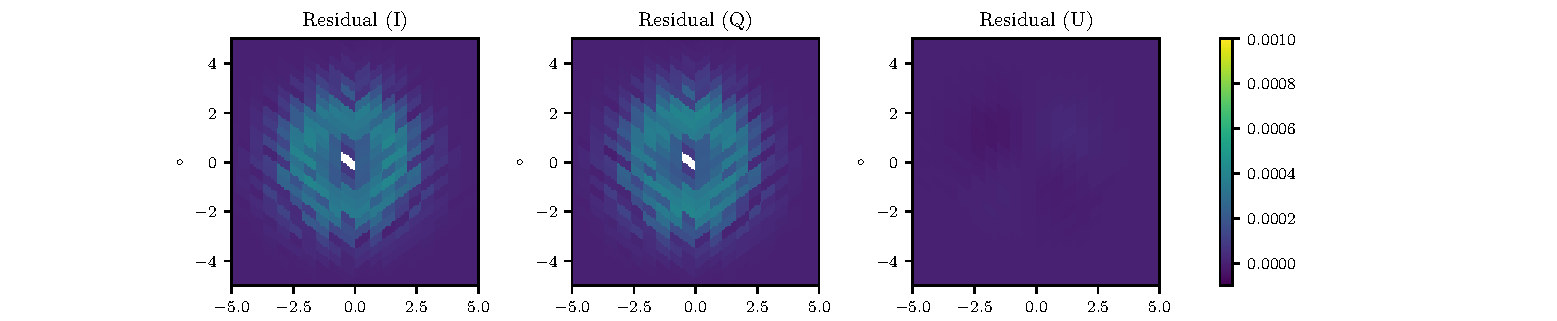
\includegraphics[width=1.0\linewidth]{figures/stokes_Q_source_256_beam_1024_dec_45.pdf}
		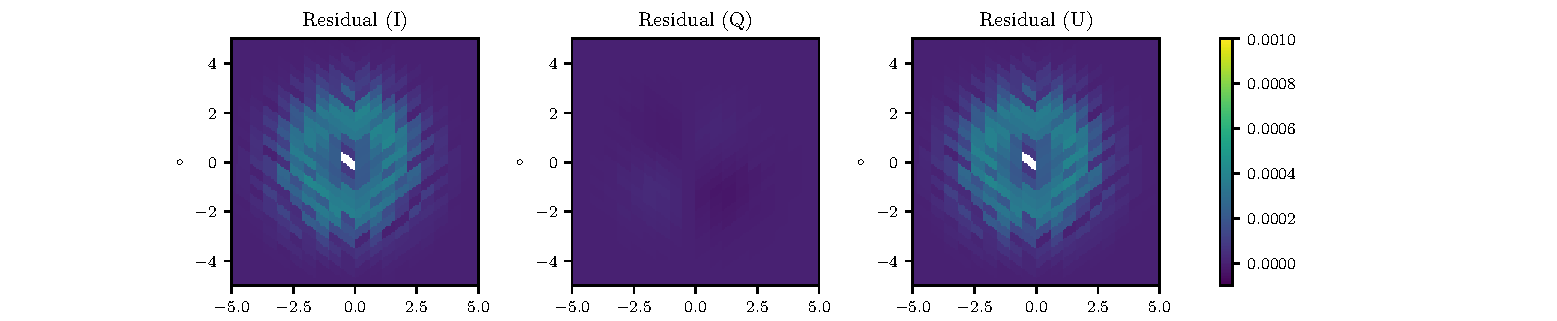
\includegraphics[width=1.0\linewidth]{figures/stokes_U_source_256_beam_1024_dec_45.pdf}
		\caption{Figure showing the results from subtracting a map of a point source convolved with a Gaussian beam using \texttt{smoothing}, and the map using generated by PISCO. Input map used HEALPix pixelization with $\mathrm{\texttt{NSIDE}} = 256$. Beamsor uses $\mathrm{\texttt{NSIDE}} = 1024$. Gaussian profile used for the beamsor had $1.5^\circ$ of Full Width at Half Maximum. All point sources are located at $45^\circ$ declination. Color scale is normalized to $1$. Plots, in order: residuals for the case of a point source with Stokes vector $S = (1,0,0,0)$, $S=(1,1,0,0)$ and $S=(1,1/\sqrt{2},1/\sqrt{2},0)$. }
		\label{fig::stokesqsource256beam1024dec45}
	\end{figure*}
	
	\subsection{Validation using mock whole sky observations}
	\label{sec::val_sky}
	This test can be summarized in the following steps
	
	\begin{itemize}
		\item Build mock CMB whole sky maps for different values of the tensor-to-scalar ratio, $r$: $0, 0.01$ and $0.1$.
		\item Set up the scanning strategy to visit each pixel at 3 different position angles $\psi_0 = 0^{\circ},45^{\circ},90^{\circ}$. The scanning uses a single detector with $\zeta=0^\circ$.
		\item Make maps of TOD generated by PISCO. 
		\item Compare the maps with a harmonic space convolution of the CMB map with a Gaussian beam.
	\end{itemize}
	
	Similarly to the point source test, the beamsor was set to be a circularly symmetric Gaussian beam with Full Width at Half Maximum of $1.5^\circ$. The resolution ratio was set to $4$, with the maps having $\mathrm{\texttt{NSIDE}} = 256$ while the beamsor used $\mathrm{\texttt{NSIDE}} = 1024$. We repeated the test using different values for $r$ to assess the capability of PISCO to recover B-modes. Particularly, $r=0$ directly tests for leakage from E-modes to B-modes or from temperature to polarization. $r=0.01$ is the current target of experiments like CLASS (\cite{2016SPIE.9914E..1KH}), while $r=0.1$ is, roughly, the current limit (see \cite{2018PhRvL.121v1301B}). As with the first test, TOD generated by PISCO do not include any noise. The scanning strategy was set to visit all pixels, so that a simpler power spectra estimator like $\texttt{anafast}$ could be used. This also guarantees the effect of incomplete sky coverage does not affect the results. 
	
	The sky model used in this test corresponds to a mock CMB. The sky model is a pure CMB, with no foregrounds are present. The maps were generated using a combination the CAMB software package (see \cite{Lewis:2002ah}) and \texttt{synfast}. Given the cosmological parameters from the latest Planck results (see \cite{2016A&A...594A..13P}), CAMB generates all 6 power spectra for an un-lensed CMB. The reason for this is that lensing produces leakage from E-modes to B-modes. The 3 sets of power spectra were generated with 3 different values of the tensor to scalar ratio, $r$: $r=0.0$ (no B-modes), $r=0.01$ and $r=0.1$. Once CAMB generated the required power spectra, we used \texttt{synfast} to create mock CMB maps in $I,Q$ and $U$. The input maps were then analyzed using \texttt{PolSpice} to obtain their power spectra, which was in turn compared to the input one to guarantee integrity.
	
	Results are shown in figure \ref{fig::pisco4wholesky}. A slight deviation with respect to the base power spectra is present at $\ell \approx 250$. We believe this discrepancy is due to the spherical bi-linear interpolation that is carried out to compute equation \ref{eq::discrete_beam_conv_tensor}. Upgrading the scheme to higher order like a spline interpolation should remove this discrepancy. Duplicating the resolution of the beamsor is expected to produce a similar result. On the other hand, there is good agreement between the output of \texttt{smoothing} and PISCO, with little or no signs of significant deviations across the $\ell=[2,200]$ span.
	
	\begin{figure*}
		\centering
		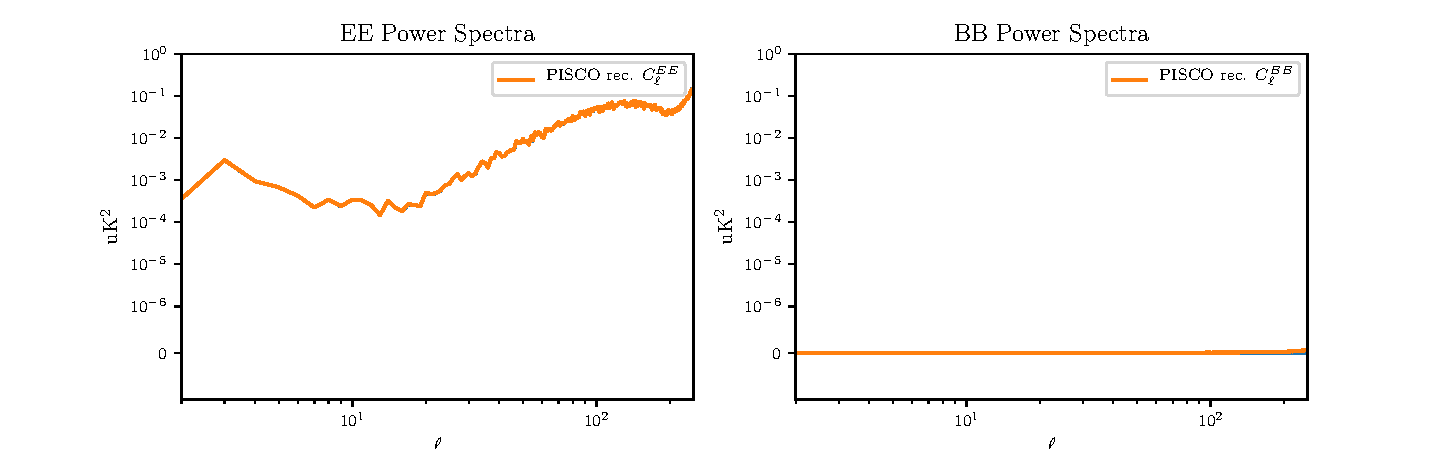
\includegraphics[width=1\linewidth]{figures/ps_r0d00.pdf}
		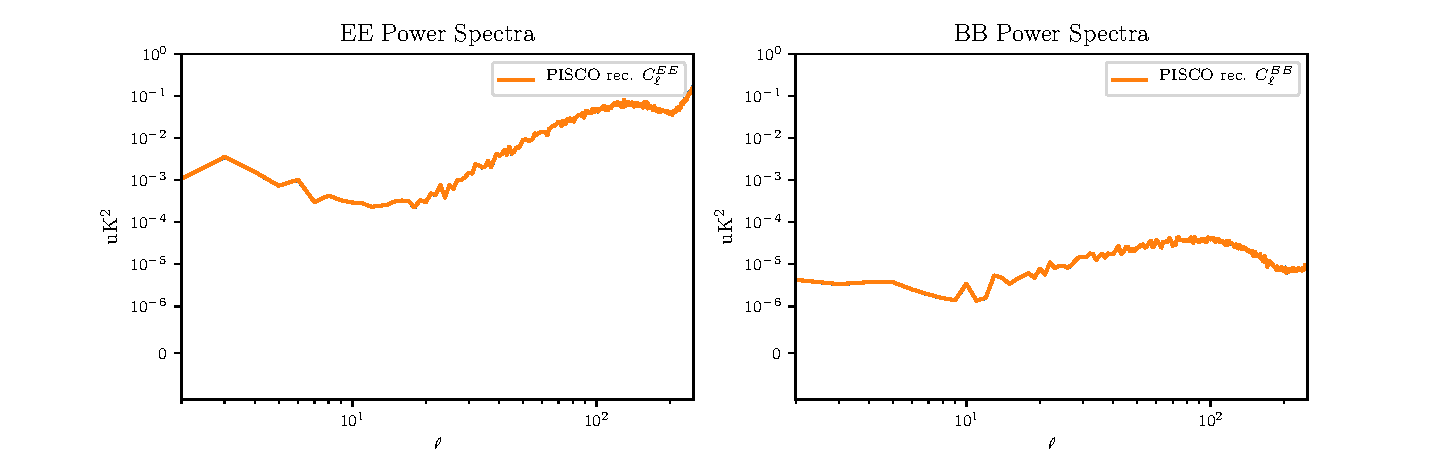
\includegraphics[width=1\linewidth]{figures/ps_r0d01.pdf}
		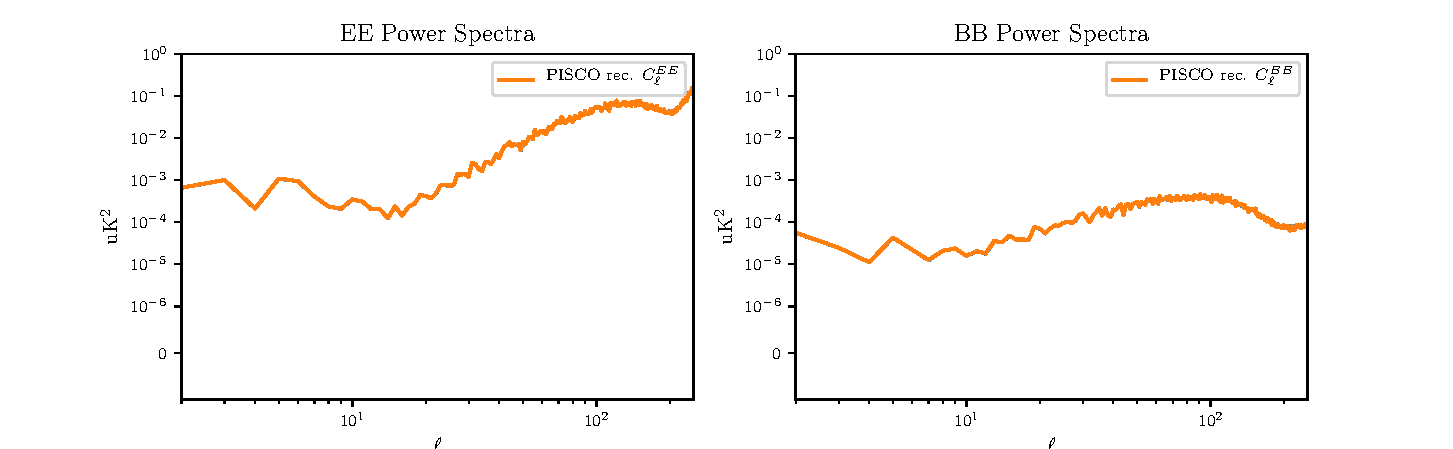
\includegraphics[width=1\linewidth]{figures/ps_r0d10.pdf}
		\caption{Plots showing maps of PISCO generated TOD and the results from \texttt{smoothing} for whole sky CMB test. Input map used HEALPix pixelization with $\mathrm{\texttt{NSIDE}} = 256$. The beamsor was also pixelated using HEALPix, but with $\mathrm{\texttt{NSIDE}} = 1024$. Maps were generated using CAMB (see \cite{Lewis:2002ah}) to generate $C_\ell$, and $\texttt{synfast}$ (part of the HEALPix package) to transform the $C_\ell$ to CMB maps. Gaussian profile used for the beamsor had $1.5^\circ$ of Full Width at Half Maximum. Different plots correspond to power spectra for input maps with values of $r=0$ (upper plot), $r=0.01$ (middle plot) and $r=0.1$ (bottom plot). Blue curve corresponds to the power spectra of the input CMB. Orange curve corresponds to the power spectra of the output maps obtained from PISCO generated TOD. No appreciable T to P or P to P leakage is present, except above $\ell \approx 250$.}
		\label{fig::pisco4wholesky}
	\end{figure*}
	
	%
	\section{Application to a CMB experiment with elliptical beams}
	\label{sec::class_pisco_sim}
	
	In this section, we show results of applying PISCO to a real CMB experiment, the Cosmology Large Angular Scale Surveyor, CLASS. The CLASS experiment is located near Llano de Chajnantor, at 5180 meters above sea level in northern Chile's Atacama Desert. CLASS aims at characterizing the large scale anisotropy of E-mode and B-mode power spectra at the $r=0.01$ level. The combination of large Field Of View (FOV) and novel optical design used by CLASS makes it an good candidate to explore the impact of beam eccentricity on the power spectra. 
	
	\subsection{Sky model}
	
	We followed a similar procedure to the one described in section \ref{sec::val_sky} to generate the maps for this simulation. Maps were generated with 3 different values of the tensor to scalar ratio, $r$: $r=0.0$ (no B-modes), $r=0.01$ (CLASS target) and $r=0.1$, roughly the current limit (see \cite{2018PhRvL.121v1301B}). CLASS Q-band has a beam with a FWHM of 1.5 degrees, so mock CMB maps are not required to be generated at higher resolution than the FWHM of the beam. The optimal resolution was found to $\mathrm{\texttt{NSIDE}} = 128$ for the maps, setting the beamsor resolution to $\mathrm{\texttt{NSIDE}} = 512$. This restricts the analysis in harmonic space to $\ell < 350$, but speeds up the computation by roughly a factor of 4. Since CLASS aims at characterization of the power spectra on large angular scales, we do not expect this constraint to affect the results significantly.
	
	\subsection{Pointing}
	
	The scanning strategy of CLASS is composed of constant elevation scans. The elevation is kept at $45^{\circ}$ while the telescope rotates $720^\circ$ in azimuth at $1$ degree per second. This process is repeated for around 18 hours per day. The boresight is rotated from $-45^{\circ}$ to $+45^{\circ}$ by $15^{\circ}$ per day on a weekly schedule. This scanning strategy ensures that more than 70 percent of the sky gets covered each day, while only 7 days are needed to provide excellent polarization angle coverage. Boresight rotation is also key to allow modulation of both $Q$ and $U$ signals (see \cite{2016SPIE.9914E..1KH}) CLASS records data $200$ times per second. Pointing streams were synthesized at $20$ Hz using the scanning strategy described above. This down-sampling factor was carefully selected so as not to produce pixel misses. 
	
	\subsection{Beamsor model}
	
	Following the work of \cite{2012SPIE.8452E..20E} and valuable input from the CLASS Collaboration, we built beamsor models for all the 72 detectors of the CLASS Q-band telescope. For simplicity, these beamsors are diagonal so that no cross-polarization is present, while the diagonal components correspond to pure elliptical Gaussian profiles. A visual representation of these fits is shown in figure \ref{fig::qbandbeamsmainbeamfwhmx}.
	
	Beamsors were saved as HEALPix with \texttt{NSIDE}$=512$. Given that CLASS Q-band is designed to have a beam with Full Width at Half Maximum of $1.5^\circ$, PISCO only considered the beam as different from zero up to $5^\circ$ away from its centroid. We chose this value because, for a unit normalized beam, a pixel that is $5^\circ$ away from beam peak would has a value of $\approx 10^{-14}$, roughly the limit of double precision floating point arithmetic. 
	
	\begin{figure}
		\centering
		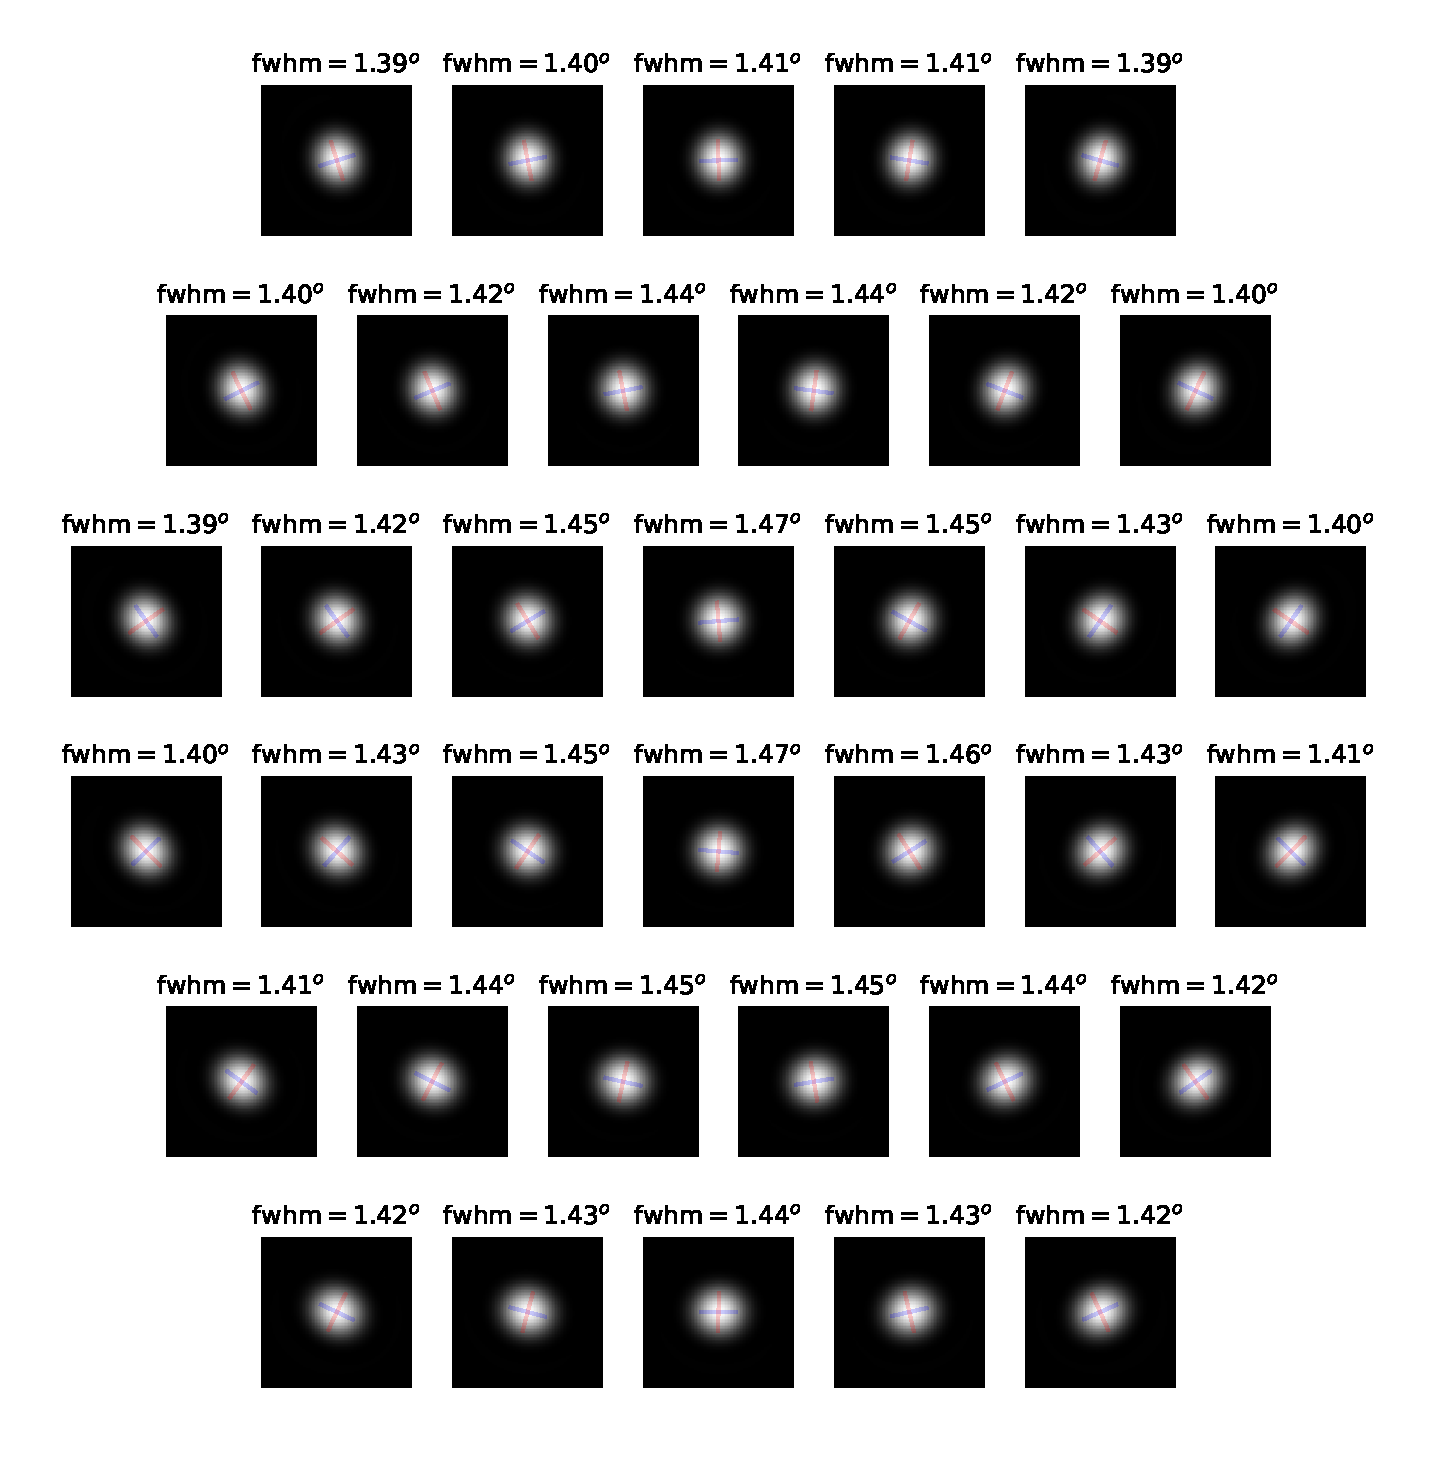
\includegraphics[width=1.0 \linewidth]{figures/qband_beams_main_beam_fwhm_x}
		\caption{Elliptical Gaussian profiles used as beamsor models for the CLASS Q-band telescope. Relative positions of plots are representative of the positions of feedhorns on the sky. In image coordinates, Zenith is up while East is to the left. All beam profiles are unit normalized, the color scale being linear. Each subplot is a plane projection on the sky of $5\times5$ square degrees. The title of each subplot is the Full Width at Half Maximum of the profile along its semi-major axis. Non negligible amounts of eccentricity can be seen in the beam profiles, and a visible correlation between feedhorn location, eccentricity and orientation of the major (minor) axis is present. Maximum eccentricity reaches $0.45$.}
		\label{fig::qbandbeamsmainbeamfwhmx}
	\end{figure}
	
	\subsection{Power spectra analysis}
	
	The power spectra of the resulting CMB map were computed using \texttt{PolSpice}\footnote{The tool that was used corresponds to the Python implementation of the SPICE algorithm by Nathan Miller.} instead of \texttt{anafast} because \texttt{PolSpice} accounts for incomplete sky coverage. Power spectra were divided by a window function corresponding to the spin-2 spherical transform of a diagonal beamsor with circularly symmetric Gaussian profiles of $1.5^\circ$ of Full Width at Half Maximum. The window function was calculated using the \texttt{gauss-beam} routine present in the \texttt{healpy} Python package.
	
	We analyzed the resulting power spectra, particularly for the B-modes, by performing a Maximum Likelihood (ML) estimation of $r$, the tensor-to-scalar ratio. While the routine in charge of this process was very simplistic, we believe it to be realistic enough to properly quantify the results of this work. Preliminary testing shows that the power spectrum is affected by incomplete sky coverage at low $\ell$. This situation can handled by using a more sophisticated power spectrum estimator.(see \cite{2015ApJ...814..103W} ) Uncertainties in the fitting procedure were estimated using a Monte-Carlo Markov Chain (MCMC), carried out using \texttt{emcee}.(\cite{emcee})
	
	\subsection{Results}
	
	Analysis of the power spectra obtained from maps that were generated from mock TOD indicate that there is an excess B-mode signal around $\ell=50$, as shown in figure \ref{fig::piscoclasssim}. Simulations show that this effect appears independent of the amplitude of the B-modes of the input CMB map. Results from the ML fits show that this excess in the B-mode signal does not significantly affect estimation of $r$.
	
	\begin{table}[width=1\linewidth,cols=2,pos=h]
		\caption{Table showing the result from fitting for $r$, the tensor-to-scalar ratio, from power spectra of maps obtained from mock data generated by PISCO. }
		\label{table::pisco_fits}
		\begin{tabular*}{\tblwidth}{@{} CC@{} }
			\toprule
			$r_\mathrm{fit}$ from PISCO output & Input value of $r$, $r_{\mathrm{in}}$ \\
			\midrule
			$0.09^{+0.02}_{-0.01}$ & $0.1$ \\
			$0.01^{+0.03}_{-0.02}$ & $0.01$ \\
			$0.0^{+0.0003}_{-0.0001}$ & $0.00$ \\ 
			\bottomrule
		\end{tabular*}
	\end{table}
	
	\begin{figure*}
		\centering
		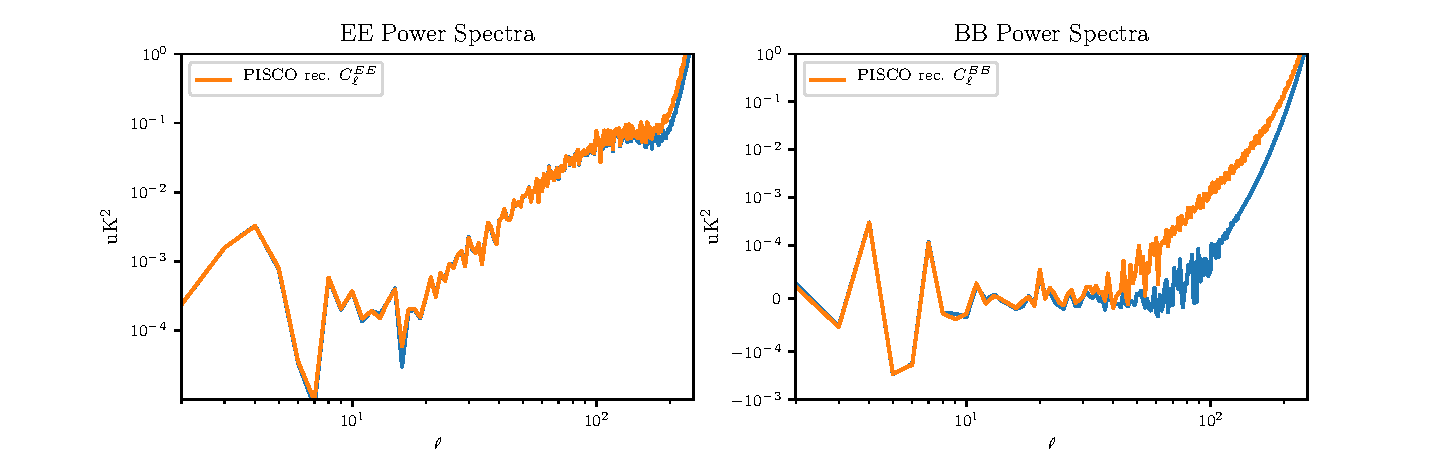
\includegraphics[width=1.0\linewidth]{figures/CLASS_scan_7_20_elliptical_gussian_beams_r_0d00.pdf}
		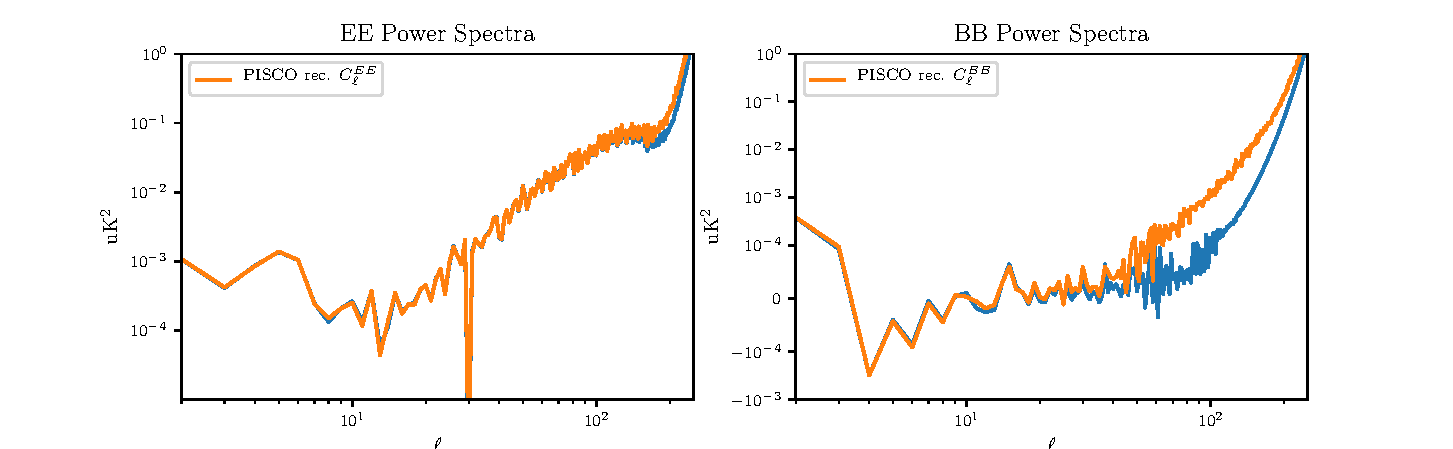
\includegraphics[width=1.0\linewidth]{figures/CLASS_scan_7_20_elliptical_gussian_beams_r_0d01.pdf}
		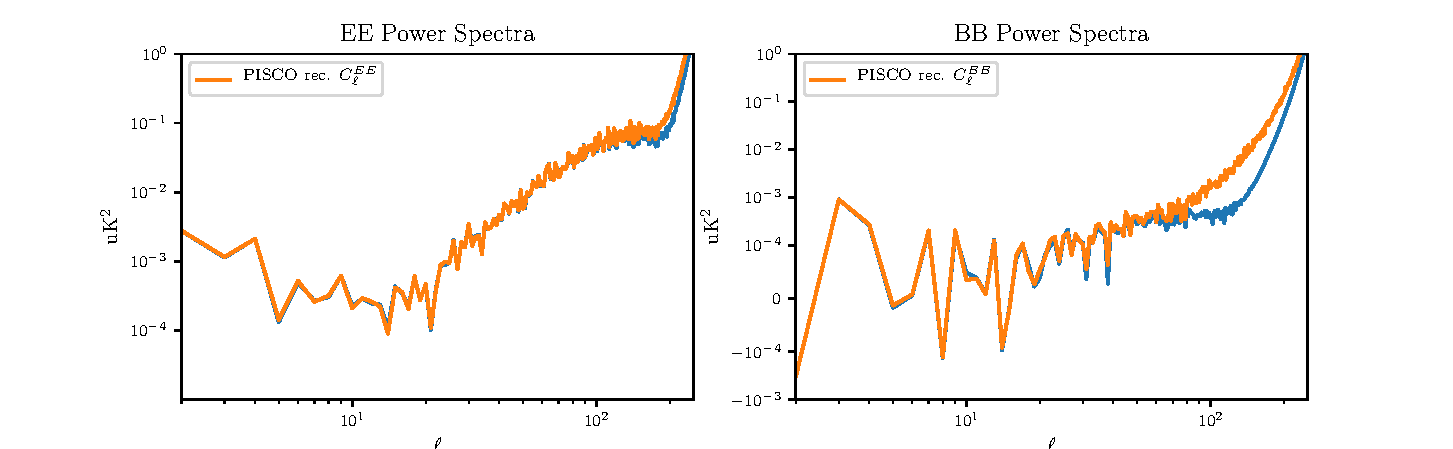
\includegraphics[width=1.0\linewidth]{figures/CLASS_scan_7_20_elliptical_gussian_beams_r_0d10.pdf}
		\caption{$EE$ and $BB$ power spectra computed from the simulated observation. In blue is the expected output power spectra of the maps as if the CMB was observed by a circularly symmetric Gaussian beam via the harmonic space convolution. In orange, the power spectra of the PISCO convolved maps, using elliptical beams. Upper plot corresponds to $r=0$, middle one to $r=0.01$ and bottom most to $r=0.1$. From visual inspection, there is good agreement with both the input power spectra and the ones computed from $\ell m$ smoothed ones. For all cases, the $BB$ power spectrum shows an excess starting at $\ell = 50$.}
		\label{fig::piscoclasssim}
	\end{figure*}
	
	\subsection{Discussion}
	
	Leakage arising from asymmetrical beams has been extensively documented. Arguments suggest that sufficient beam rotation with respect to the sky basis helps suppress the effect of beam asymmetry (see \cite{2003ApJS..148...39P}). This is because if each pixel is visited at all possible beam orientations, the \textsl{effective beam} at that pixel will be symmetrical, no matter what the ``instrumental'' beam is. As described in \cite{2007MNRAS.376.1767O}, a similar effect arises when considering beamsors. It is then natural to consider leakage to be caused by a combination beam asymmetry and incomplete beam rotation.
	
	The results from the previous section suggest that beam asymmetry causes an excess B-mode signal. Since the amplitude of the apparent leakage appears to be independent of the value of $r$, we believe leakage is of T to P type. This hypothesis can be checked by repeating the simulation using an unpolarized CMB; if no T to P leakage is present, the resulting E-mode and B-mode power spectra will be zero.
	
	We repeated the simulation described in the previous section, using an unpolarized CMB as input. The resulting power spectra are shown in figure  \ref{fig::classscan720circulargaussianbeamsr0d00extratonly}. Power spectra show a nonzero E-mode and B-mode signal, which indicates the type of leakage to be temperature to polarization.
	
	\begin{figure*}
		\centering
		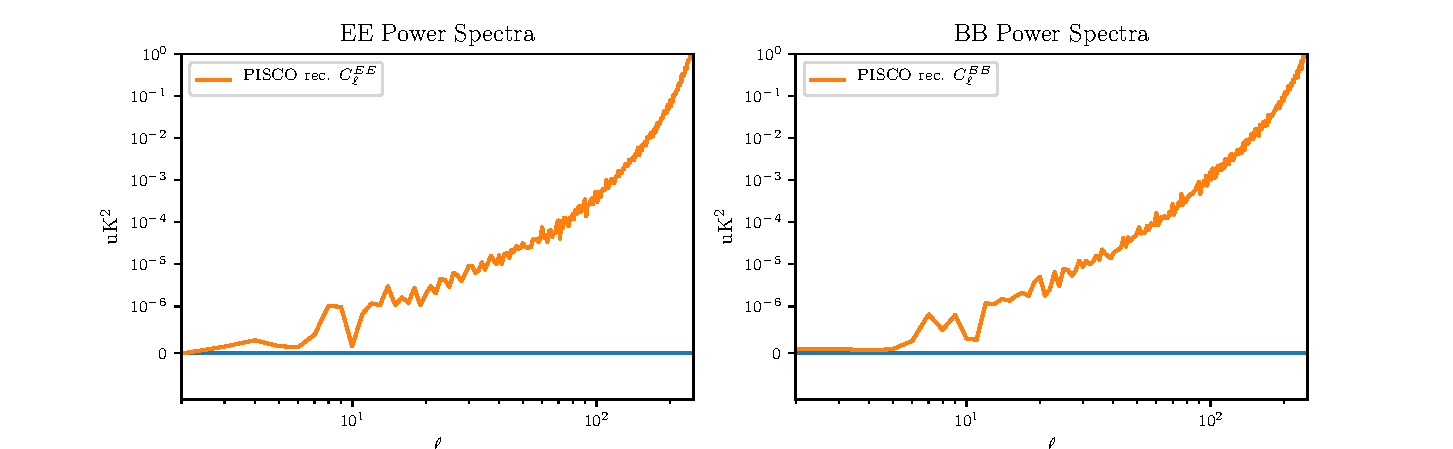
\includegraphics[width=1.0\linewidth]{figures/T_to_P_leakage_for_class.pdf}
		\caption{Power spectra for temperature, E-mode and B-mode components of maps generated using synthetic TOD. The simulation was similar to one described in \ref{sec::class_pisco_sim}, except that the input CMB is unpolarized. This last condition ensures that any polarization signal present in the output maps is due to the effect of beam asymmetry.}
		\label{fig::classscan720circulargaussianbeamsr0d00extratonly}
	\end{figure*}
	
	
	\section{Conclusion}
	\label{sec::conclusions}
	
	In this work, we have presented PISCO, a new computer simulation code capable of computing tensor convolutions in pixel space for applications in CMB experiments. PISCO was also designed to use GPU acceleration, as well as supporting execution on HPC facilities. PISCO is also unique in its field, being capable of explicitly including time-dependent phenomena present in the data, like modulation techniques, beam degradation due to mechanical effects and transient events on the sky. Application of these capabilities to a realistic CMB experiment will be given in future publications.
	
	This work also showed an application of PISCO to the CLASS experiment and its Q-band telescope. Using a reasonable representation of the beams and scanning strategy, we found that an experiment like CLASS Q-band should experience T to P leakage on its power spectra. T to P leakage is expected in the case of experiments with asymmetrical beams. We believe this result is a strong indication that more work is needed in order to fully understand the effects of beam asymmetry for the CLASS experiment, with future applications taking into account VPM modulation, realistic sky models, stochastic and systematic noise sources and more accurate models of the beams.
	
	%\section*{References}
	
	\bibliographystyle{model2-names}
	\bibliography{bib}

	\appendix
	%\numberwithin{equation}{section}	
	\section{Computation of antenna coordinates from sky coordinates and antenna pointing}
	
	In this appendix we introduce an additional coordinate system, the \textsl{instrument basis} which is a spherical coordinate system with unit base vectors $\hat{x}'$, $\hat{y}'$ and $\hat{z}'$ and spherical coordinates $\theta'$ and $\phi'$. For any given beam center pointing $\bar{q}_0$ in the sky basis, the pointing direction unit vector $\hat{p}_0$ points to the sky at the equator and prime meridian $(\theta_0',\phi_0') = (90,0)$ so that the unit vectors $\hat{\theta}_0'$ and $\hat{\phi}_0'$ at that point form the unit base vectors of the antenna basis coordinate system. It is natural for PISCO to adopt Ludwig's 2nd definition of cross polarization \cite{1140406} as this aligns the unit vectors $(\hat{e}_{\co},\hat{e}_{\cx})$ with $(\hat{\theta}',\hat{\phi}')$ for a detector with orientation angle $\zeta = 0$. In particular, this means that, for any beam center pointing $\bar{q}_0 = (90,\phi,0)$ in the sky basis, the co and cross polarization unit vectors are aligned with the Stokes parameters $+U$ and $-U$ respectively across the entire sky.
	
	For a beam center pointing $\bar{q}_0$ and off beam center pointing $\bar{q}$ in the sky basis, we can derive the antenna basis coordinates $(\rho,\sigma)$ and angle $\psi$ between $\hat{e}_{\co}$ and $+U$ ($\hat{\theta}$) by using spherical trigonometry (see Figure \ref{fig::figure10}). 
	
	\begin{figure}
		\centering
		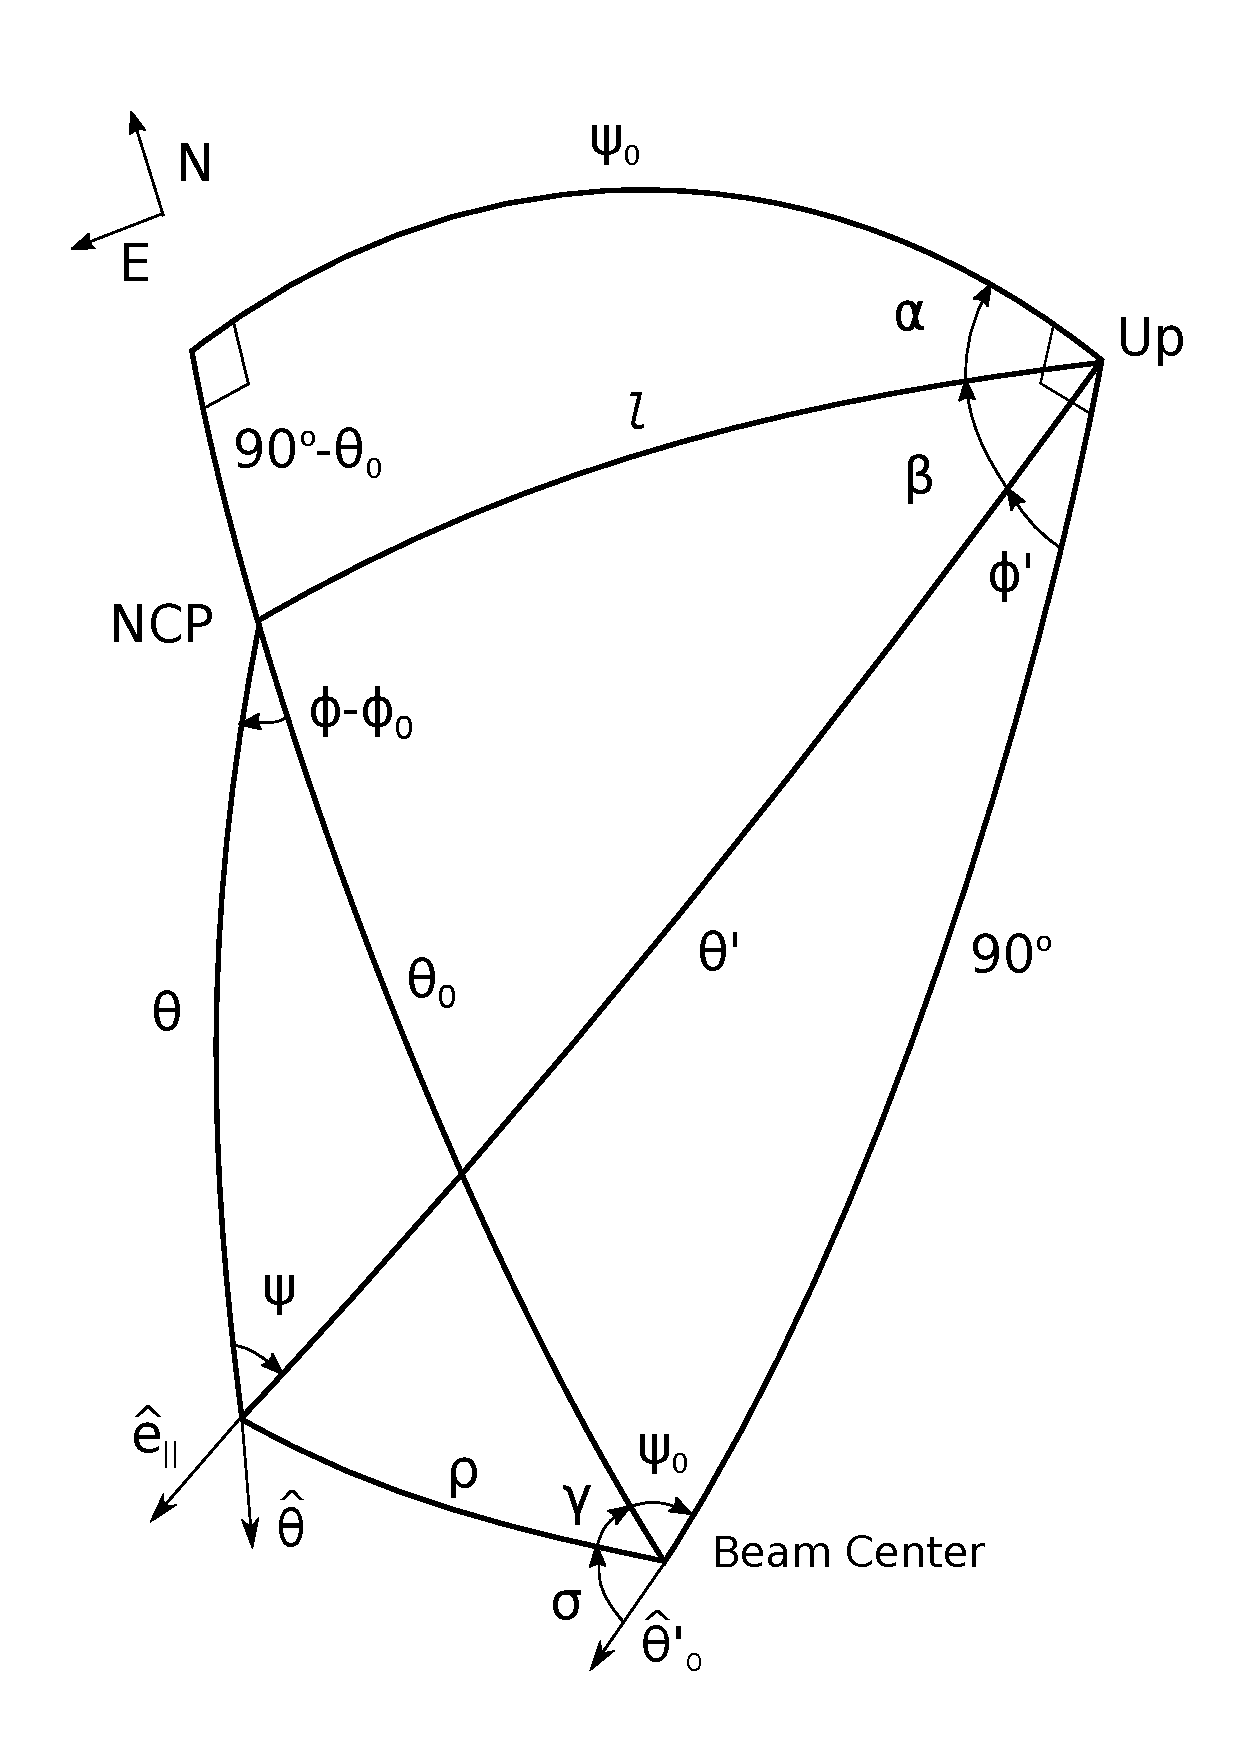
\includegraphics[width=1.0\linewidth]{figures/Figure10.pdf}
		\caption{Sky, instrument and antenna basis coordinates for beam center pointing $\bar{q_0}$ and off beam center pointing $\bar{q}$. Here $\mathrm{\texttt{NCP}}$ is the ICRS North Celestial Pole and $\mathrm{\texttt{Up}}$ is the pole in the up direction of the instrument basis coordinate system. The arc $l$ is the analog of the ITRS co-latitude.}
		\label{fig::figure10}
	\end{figure}
	
	Defining $\Delta \phi \equiv \phi - \phi_0$, the antenna basis coordinates $(\rho,\sigma)$ are given by
	%
	\begin{flalign}
	\rho  &= \arccos( \cos(\theta) cos(\theta_0) + \sin(\theta) \sin(\theta_0) \cos(\Delta \phi) ) \nonumber & \\
	\sin(\gamma) &= \frac{\sin(\theta) \sin(\Delta \phi)}{\sin(\rho)} \nonumber & \\
	\cos(\gamma) &= \frac{\cos(\theta) \sin(\theta_0) - \sin(\theta) \cos(\theta_0) \cos(\Delta \phi)}{\sin(\rho)} & \\ 
	\gamma       &=  \arctan \left(\frac{\sin(\theta) \sin(\Delta \phi)}{\cos(\theta) \sin(\theta_0) - \sin(\theta) \cos(\theta_0) \cos(\Delta \phi)} \right) \nonumber & \\
	\sigma &= 180^{\circ} - \psi_0 - \gamma \nonumber &
	\end{flalign}
	%
	Then the instrument basis coordinates $(\theta', \phi')$ are
	%
	\begin{flalign}
	\theta' &= \arccos(-\sin(\rho) \cos(\sigma)) \nonumber & \\
	\sin(\phi') &= \frac{\sin(\rho) \sin(\sigma)}{\sin(\theta')} \nonumber & \\
	\cos(\phi') &= \frac{\cos(\rho)}{\sin(\theta')} & \\
	\phi'       &= \arctan \left( \frac{\sin(\rho) \sin(\sigma)}{\cos(\rho)} \right) \nonumber &
	\end{flalign}
	%
	From the uppermost spherical triangle in figure \ref{fig::figure10}, we have
	%
	\begin{flalign}
	\cos(l) &= \sin(\theta_0) \cos(\psi_0) \nonumber & \\
	\sin(\alpha) &= \frac{\cos(\theta_0)}{\sin(l)} \nonumber & \\ 
	\cos(\alpha) &= \frac{\sin(\theta_0)  \sin(\psi_0)}{\sin(l)}  & \\
	\alpha       &= \arctan\left( \frac{\cos(\theta_0)}{\sin(\theta_0)  \sin(\psi_0)} \right) \nonumber &
	\end{flalign}
	%
	This yields
	%
	\begin{flalign}
	\beta &= 90^{\circ} - \alpha - \phi' \nonumber & \\
	\cos(\psi) &= \frac{\cos(l) \sin(\theta') - \sin(l) \cos(\theta') \cos(\beta)}{\cos(\theta)}  \nonumber & \\
	\sin(\psi) &= \frac{\sin(l) \sin(\beta)}{\cos(\theta)}  & \\
	\psi       &= \arctan\left( \frac{\sin(l) \sin(\beta)}{\cos(l) \sin(\theta') - \sin(l) \cos(\theta') \cos(\beta)} \right)  \nonumber &
	\end{flalign}
	
	\section{Calculation of elements of $B$}
	
	A beamsor $B$ evaluated at antenna basis coordinates $(\rho,\sigma)$ is a $4 \times 4$ matrix with elements
	
	\begin{equation}
	\begin{aligned}
	B(\rho,\sigma) = \frac{1}{\tilde{\Omega}}
	\begin{bmatrix}
	B_{TT} & B_{QT} & B_{UT} & B_{VT}\\
	B_{TQ} & B_{QQ} & B_{UQ} & B_{VQ}\\
	B_{TU} & B_{QU} & B_{UU} & B_{VU}\\
	B_{TV} & B_{QV} & B_{UV} & B_{VV}
	\end{bmatrix}
	\end{aligned}
	\label{eq::beamsor_appendix}
	\end{equation}
	
	\noindent
	with $\tilde{\Omega}$ being a normalization factor computed as
	
	\begin{equation}
	\begin{aligned}
	\tilde{\Omega} = \int_{4\pi} B_{TT}(\rho,\sigma) \, \mathrm{d} \Omega
	\end{aligned}
	\end{equation}
	
	The definition of a beamsor used in this work differs from the one listed in \cite{2007MNRAS.376.1767O} in that element $B_{XY}$ corresponds to element $B_{YX}$. We believe this definition yields a clearer interpretation of beamsor elements. Consider, for instance, the product of $B$ with a Stokes vector representing an unpolarized source. This yields
	
	\begin{equation}
	\begin{aligned}
	\begin{bmatrix} 
	B_{TT} \\ 
	B_{TQ} \\ 
	B_{TU} \\ 
	B_{TV} 
	\end{bmatrix}
	=
	\begin{bmatrix}
	B_{TT} & B_{QT} & B_{UT} & B_{VT}\\
	B_{TQ} & B_{QQ} & B_{UQ} & B_{VQ}\\
	B_{TU} & B_{QU} & B_{UU} & B_{VU}\\
	B_{TV} & B_{QV} & B_{UV} & B_{VV}
	\end{bmatrix}
	\cdot
	\begin{bmatrix} 
	1 \\ 
	0 \\ 
	0 \\ 
	0 
	\end{bmatrix}
	\end{aligned}
	\label{eq::unpol_beamsor}
	\end{equation}
	
	\noindent
	where it is more evident that elements $B_{TX}$, with $X=Q,U,V$, correspond to the temperature to polarization leakage beams. 
	
	In most CMB applications, linearly polarized detectors are placed at the focus of the antenna. In general, power that was radiated as pure $+Q$ in the detector basis will reach the sky as both $+Q$ and $-Q$ in the antenna basis. This effect can be modeled by introducing co-polar and cross-polar beams. The co-polar beam, $b_{\co}(\rho,\sigma)$, is the unit-normalized power density distribution that reaches the sky with a polarization state parallel to $\hat{e}_{\co}$. The cross-polar $b_{\cx}(\rho,\sigma)$ does so parallel to $\hat{e}_{\cx}$. 
	
	The work of \cite{2007A&A...470..771J} also provides a way of calculating beamsor elements. Given the coordinate system convention used in this work, it is important to re-specify the way these elements are calculated. We start by considering the antenna to broadcast power originated by a linearly polarized source radiating at the location of the detection device. This will produce a distribution of electric fields in the far field, $\vec{E} = \vec{E}(\rho,\sigma)$, where $\vec{E}(\rho,\sigma)$ will have co-polarized and cross polarized components. Take $x$ to be a source oriented such that most of its radiated power reaches the sky as electric fields aligned with $\hat{\theta}'$ at beam center. Similarly, consider another source, $y$, aligned perpendicularly such that most its transmitted power reaches the sky as electric fields aligned with $\hat{\phi}'$, at beam center. In this situation, elements of a beamsor can be computed via
	
	\begin{equation}
	\begin{split}
	B_{TT}&=\frac{1}{2}\left(\left|\vec{E}_{x}\right|^{2}+\left|\vec{E}_{y}\right|^{2}\right)\\
	B_{QT}&=\frac{1}{2}\left(\left|\vec{E}_{x,\co}\right|^{2}-\left|\vec{E}_{x,\cx}\right|^{2} +  \left|E_{y,\cx}\right|^{2}-\left|E_{y,\co}\right|^{2}\right)\\
	B_{UT}&=\frac{1}{2}\left(\vec{E}_{x,\co} E_{x,\cx}^{*} - E_{y,\co} E_{y,\cx}^{*}\right) + \mathrm{c.c.}\\
	B_{VT}&=\frac{1}{2}\mathrm{i}\left(\vec{E}_{x,\co}\vec{E}_{x,\cx}^{*} + \vec{E}_{y,\co} \vec{E}_{y,\cx}^{*}\right) + \mathrm{c.c.}\\
	B_{TQ}&=\frac{1}{2}\left(\left|\vec{E}_{A}\right|^{2}-\left|\vec{E}_{B}\right|^{2}\right)\\
	B_{QQ}&=\frac{1}{2}\left(\left|\vec{E}_{x,\co}\right|^{2}-\left|\vec{E}_{x,\cx}\right|^{2}+\left|\vec{E}_{y,\co}\right|^{2}-\left|\vec{E}_{y,\cx}\right|^{2}\right)\\
	B_{UQ}&=\frac{1}{2}\left(\vec{E}_{x,\co} \vec{E}_{x,\cx}^{*} + \vec{E}_{y,\co} \vec{E}_{y,\cx}^{*}\right)+\mathrm{c.c.}\\
	B_{VQ}&=\frac{1}{2}\mathrm{i}\left( \vec{E}_{x,\co} E_{x,\cx}^{*} - E_{y,\co} E_{y,\cx}^{*}\right)+\mathrm{c.c.}\\
	B_{TU}&=\frac{1}{2}\left( -\vec{E}_{x,\co} \vec{E}_{x,\cx}^{*} + \vec{E}_{y,\cx} \vec{E}_{y,\co}^{*}\right)+\mathrm{c.c.}\\
	B_{QU}&=\frac{1}{2}\left(-\vec{E}_{x,\co}\vec{E}_{y,\cx}^{*} - \vec{E}_{x,\cx} \vec{E}_{y,\co}^{*}\right)+\mathrm{c.c.}\\
	B_{UU}&=\frac{1}{2}\left(\vec{E}_{x,\co} \vec{E}_{y,\co}^{*} - \vec{E}_{x,\cx} \vec{E}_{y,\cx}^{*}\right)+\mathrm{c.c.}\\
	B_{VU}&=\frac{1}{2}\mathrm{i}\left(\vec{E}_{x,\co} \vec{E}_{y,\co}^{*} + \vec{E}_{x,\cx}\vec{E}_{y,\cx}^{*}\right)+\mathrm{c.c.}\\
	B_{TV}&=\frac{1}{2}\mathrm{i}\left(\vec{E}_{x,\co} \vec{E}_{y,\cx}^{*} - \vec{E}_{x,\cx}\vec{E}_{y,\co}^{*}\right)+\mathrm{c.c.}\\
	B_{QV}&=\frac{1}{2}\mathrm{i}\left(\vec{E}_{\mathrm{x,\co}} \vec{E}_{y,\cx}^{*} + \vec{E}_{x,\cx} \vec{E}_{y,\co}^{*}\right)+\mathrm{c.c.}\\
	B_{UV}&=\frac{1}{2}\mathrm{i}\left(-\vec{E}_{x,\co} \vec{E}_{y,\co}^{*} + \vec{E}_{A,\cx} \vec{E}_{y,\cx}^{*}\right)+\mathrm{c.c.}\\
	B_{VV}&=\frac{1}{2}\left(\vec{E}_{x,\co} \vec{E}_{y,\co}^{*} + \vec{E}_{x,\cx} \vec{E}_{y,\cx}^{*}\right)+\mathrm{c.c.}
	\end{split}
	\end{equation}
	%
	\noindent
	where c.c. stands for complex conjugate.
	
\end{document}
